\section{Results}
\label{sec:results}

We present results from 8{,}640 cross-validated experiments spanning three datasets, four featurisers, three surrogates, and three PCA dimensionalities.
Unless stated otherwise, all numbers refer to $\ntrain = 500$.

\subsection{Featurizer Ranking Across Datasets}
\label{sec:featurizer_ranking}

Figure~\ref{fig:bar_r2_all} presents bar charts of averaged \Rtwo{} for all featuriser--surrogate combinations across the three datasets.
ORB embeddings consistently rank first on every dataset and every surrogate.

\begin{figure*}[!htb]
    \centering
    \begin{subfigure}[t]{0.32\textwidth}
        \centering
        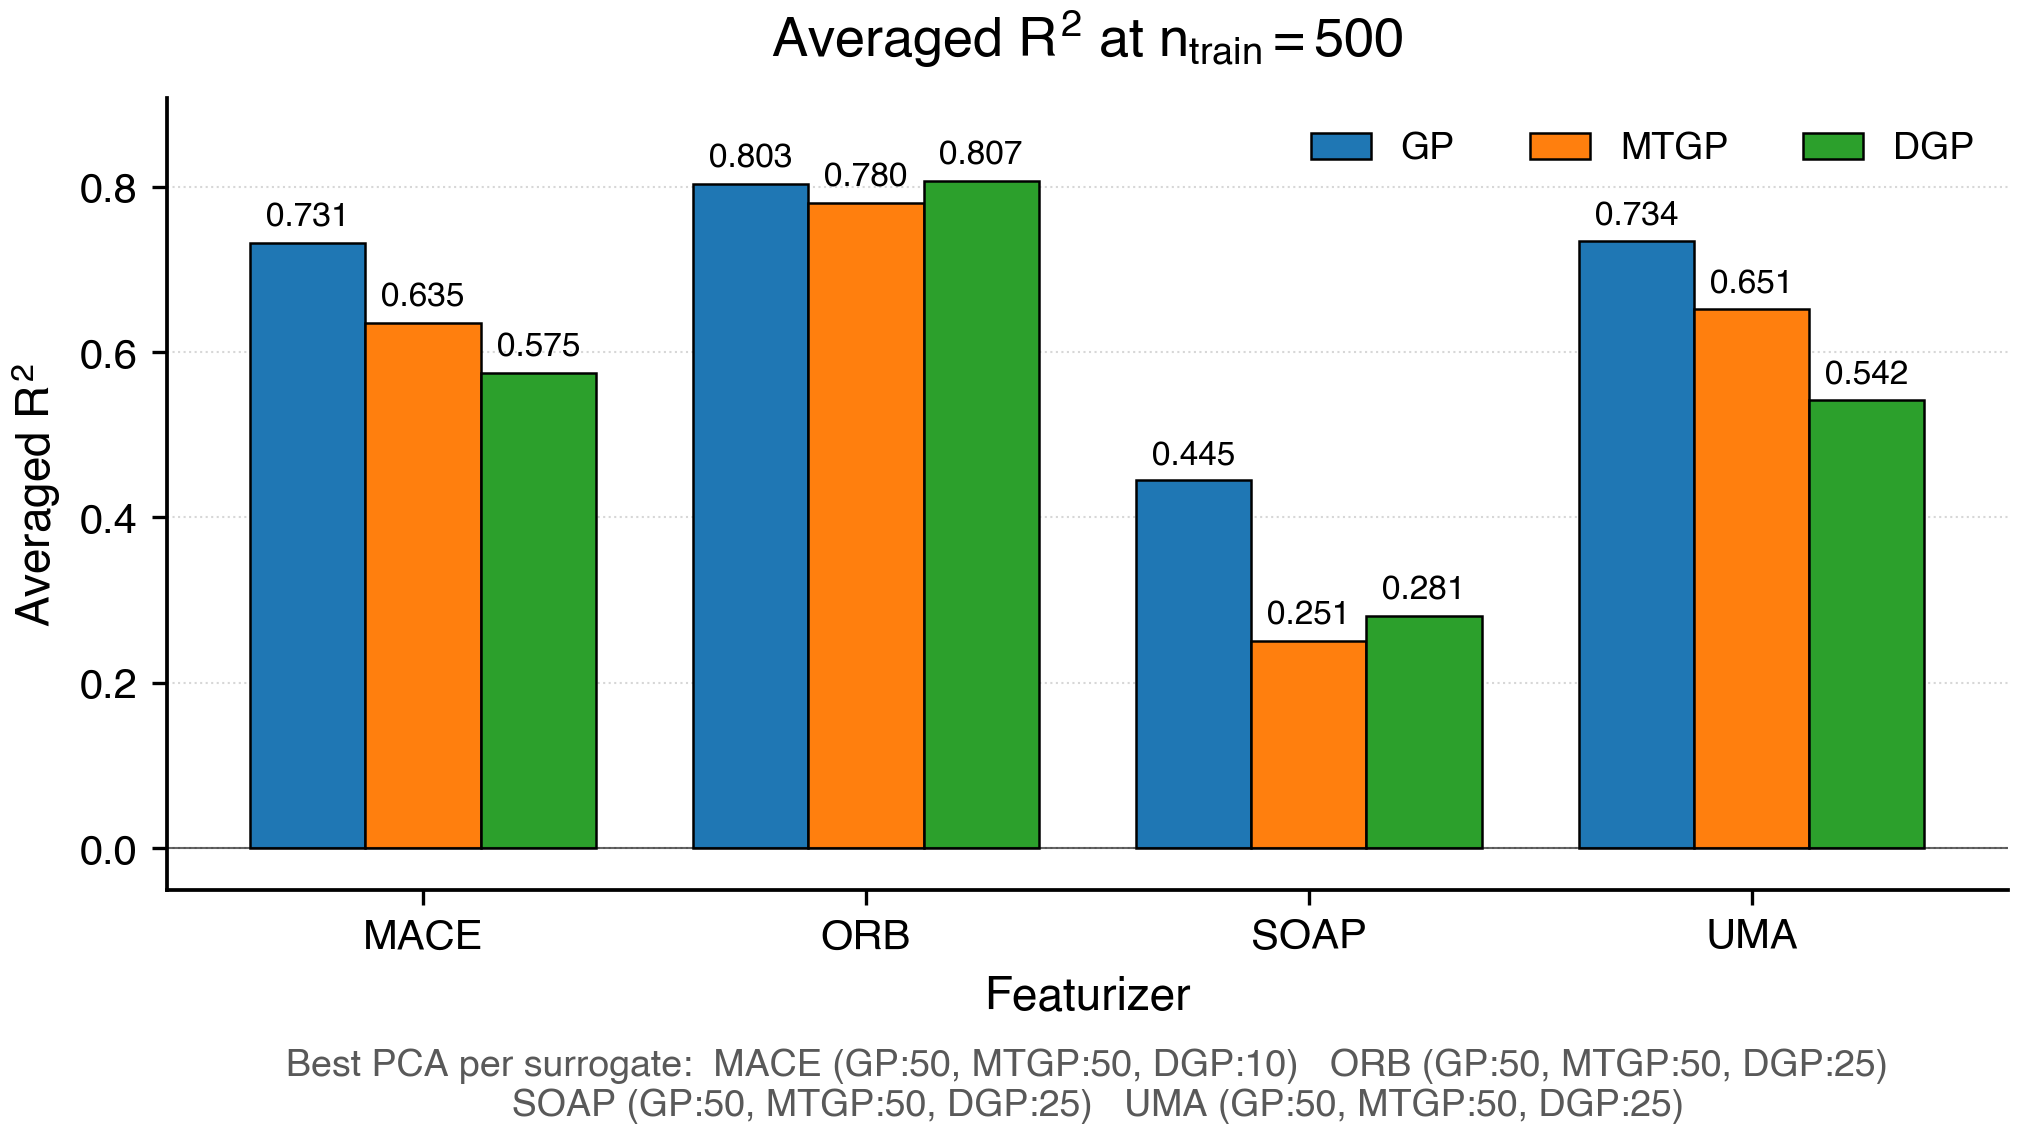
\includegraphics[width=\textwidth]{figures/fig2_bar_elastic_R2_grouped.png}
        \caption{Elastic tensor (8 properties)}
        \label{fig:bar_elastic}
    \end{subfigure}
    \hfill
    \begin{subfigure}[t]{0.32\textwidth}
        \centering
        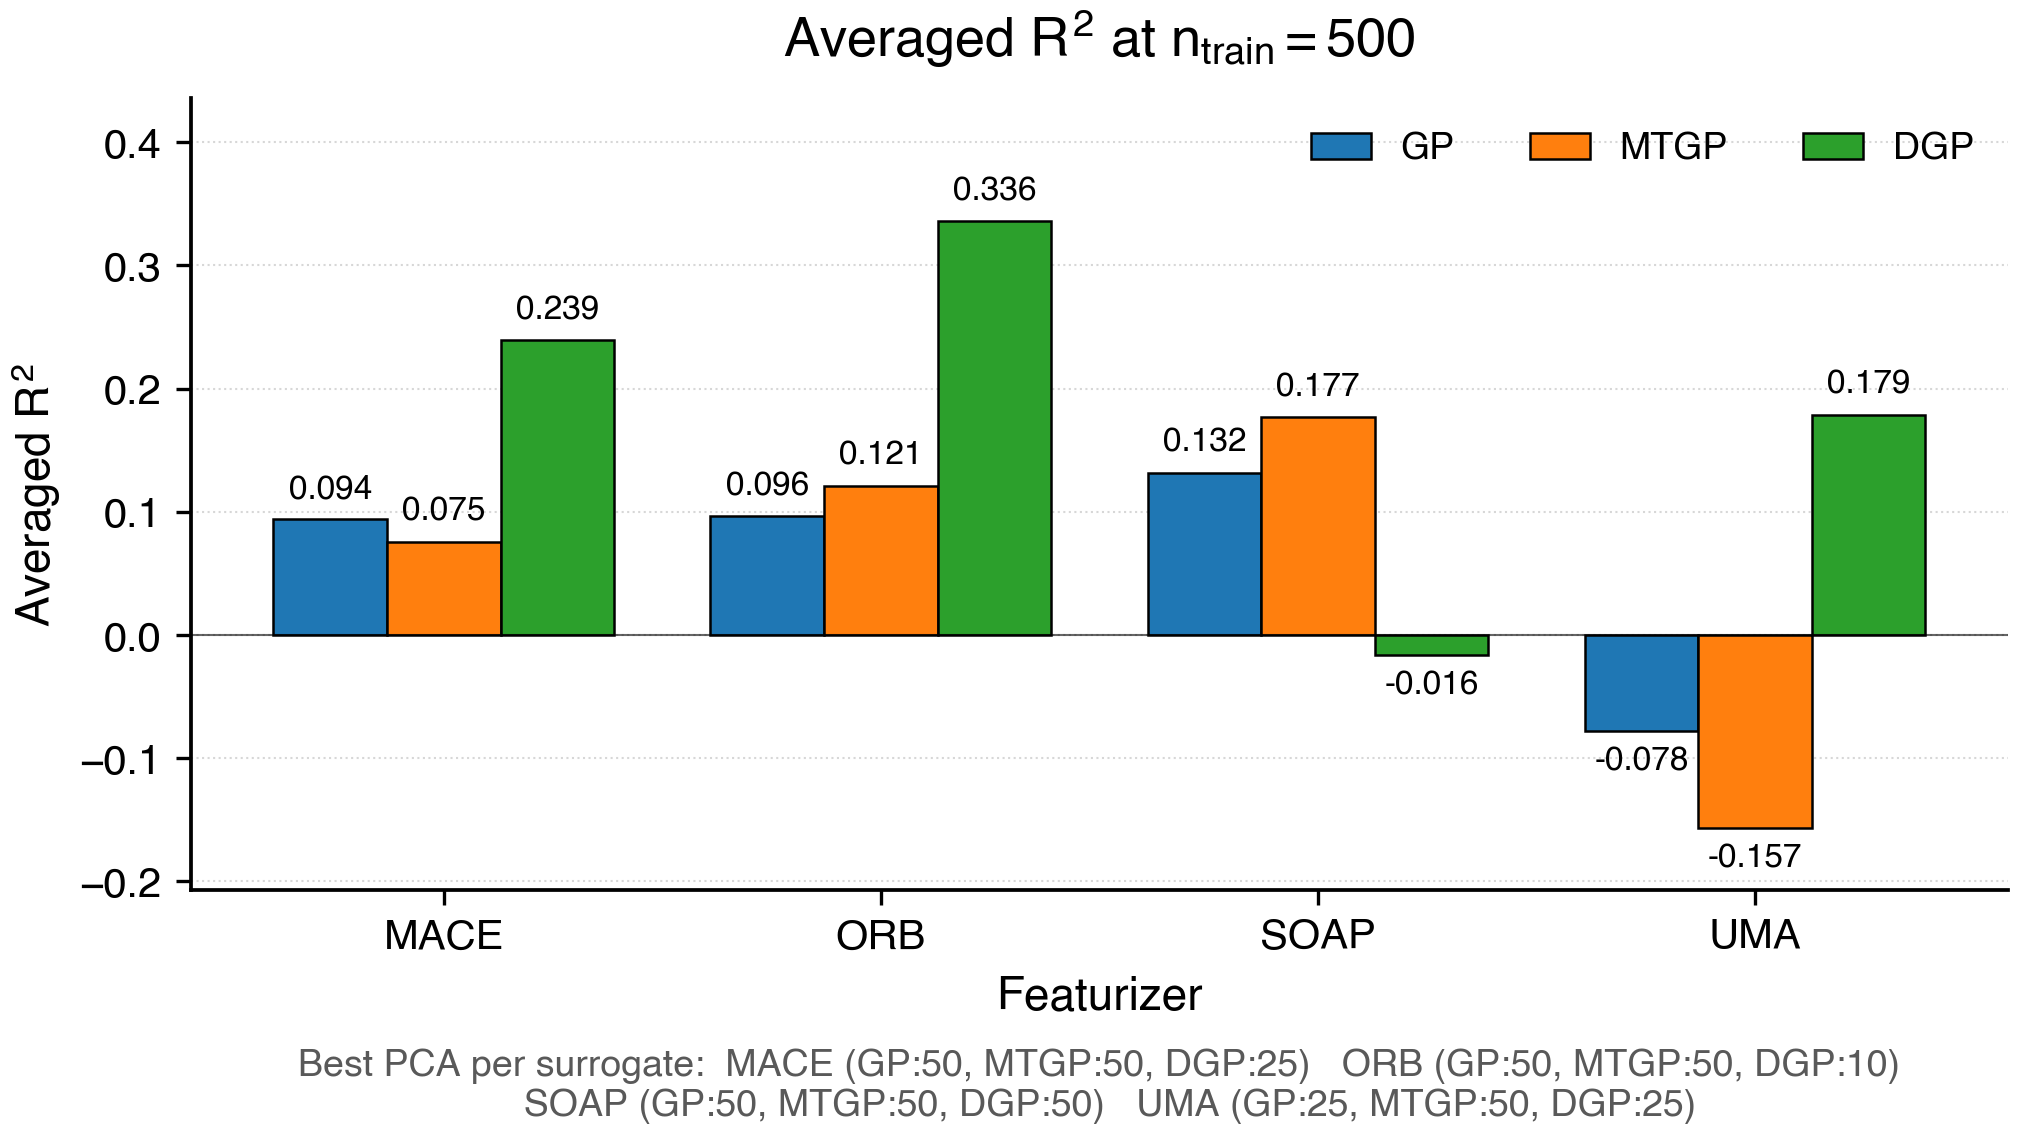
\includegraphics[width=\textwidth]{figures/fig2_bar_dielectric_R2_grouped.png}
        \caption{Dielectric constant (4 properties)}
        \label{fig:bar_dielectric}
    \end{subfigure}
    \hfill
    \begin{subfigure}[t]{0.32\textwidth}
        \centering
        
\includegraphics[width=\textwidth]{figures/fig2_bar_phonon_R2_grouped.png}
        \caption{Phonon dielectric (3 properties)}
        \label{fig:bar_phonon}
    \end{subfigure}
    \caption{Averaged \Rtwo{} across all target properties at $\ntrain = 500$, grouped by featuriser and surrogate model, for each of the three benchmark datasets. ORB embeddings dominate on all datasets. Note the different $y$-axis scales reflecting the vastly different prediction difficulty across domains.}
    \label{fig:bar_r2_all}
\end{figure*}

Table~\ref{tab:best_configs_elastic} reports the best configuration per featuriser--surrogate pair on the elastic tensor dataset.
The best overall configuration is ORB\,+\,DGP at PCA\,=\,25, achieving an averaged \Rtwo{} of 0.807 across all 8~elastic properties.
ORB\,+\,GP at PCA\,=\,50 is a close second at 0.803, with the critical advantage of far greater stability (Section~\ref{sec:pca_sensitivity}).
The featuriser ranking is remarkably consistent: ORB~($\bar{R}^2 \approx 0.80$) $>$ UMA~($\approx 0.73$) $\approx$ MACE~($\approx 0.73$) $\gg$ SOAP~($\approx 0.44$) for GP, with similar orderings for MTGP and DGP.

\begin{table*}[!htb]
    \centering
    \caption{Best configuration per featuriser--surrogate pair on the elastic tensor dataset ($\ntrain = 500$). For each combination, we report the PCA dimensionality that maximises averaged \Rtwo{} across all 8~properties, together with the corresponding averaged RMSE and Spearman~$\rho$.}
    \label{tab:best_configs_elastic}
    \small
    \begin{tabular}{@{}llcccc@{}}
        \toprule
        \textbf{Surrogate} & \textbf{Featurizer} & \textbf{Best PCA} & \textbf{Avg.\ \Rtwo{}} & \textbf{Avg.\ RMSE} & \textbf{Avg.\ Spearman} \\
        \midrule
        \multirow{4}{*}{GP}
        & ORB     & 50 & \textbf{0.803} & \textbf{17.37} & \textbf{0.842} \\
        & UMA     & 50 & 0.734 & 21.42 & 0.811 \\
        & MACE    & 50 & 0.731 & 20.46 & 0.820 \\
        & SOAP    & 50 & 0.445 & 33.63 & 0.688 \\
        \midrule
        \multirow{4}{*}{MTGP}
        & ORB     & 50 & \textbf{0.780} & \textbf{19.30} & \textbf{0.843} \\
        & UMA     & 50 & 0.651 & 25.80 & 0.780 \\
        & MACE    & 50 & 0.635 & 25.76 & 0.758 \\
        & SOAP    & 50 & 0.251 & 41.34 & 0.529 \\
        \midrule
        \multirow{4}{*}{DGP}
        & ORB     & 25 & \textbf{0.807} & \textbf{17.84} & \textbf{0.826} \\
        & MACE    & 10 & 0.575 & 25.53 & 0.659 \\
        & UMA     & 25 & 0.542 & 26.80 & 0.696 \\
        & SOAP    & 25 & 0.281 & 38.78 & 0.521 \\
        \bottomrule
    \end{tabular}
\end{table*}

Tables~\ref{tab:best_configs_dielectric} and~\ref{tab:best_configs_phonon} present the equivalent results for the dielectric and phonon datasets.
On the dielectric dataset, overall \Rtwo{} values are substantially lower, reflecting the difficulty of predicting electronic properties from geometric embeddings.
The best configuration is DGP\,+\,ORB at PCA\,=\,10 ($\bar{R}^2 = 0.336$, $\bar{\rho} = 0.778$).
Notably, SOAP is competitive on this dataset (MTGP\,+\,SOAP achieves $\bar{R}^2 = 0.177$), suggesting that the classical descriptor captures some local chemistry information relevant to dielectric response that foundation model embeddings emphasise less.

\begin{table}[H]
    \centering
    \caption{Best configuration per featuriser--surrogate pair on the dielectric constant dataset ($\ntrain = 500$).}
    \label{tab:best_configs_dielectric}
    \footnotesize
    \begin{tabular}{@{}llcccc@{}}
        \toprule
        \textbf{Surr.} & \textbf{Feat.} & \textbf{PCA} & \textbf{\Rtwo{}} & \textbf{RMSE} & \textbf{$\rho$} \\
        \midrule
        \multirow{4}{*}{GP}
        & SOAP    & 50 & 0.132 & 7.60 & 0.549 \\
        & ORB     & 50 & 0.096 & 7.84 & \textbf{0.746} \\
        & MACE    & 50 & 0.094 & 7.94 & 0.695 \\
        & UMA     & 25 & $-$0.078 & 8.14 & 0.609 \\
        \midrule
        \multirow{4}{*}{MTGP}
        & SOAP    & 50 & \textbf{0.177} & \textbf{7.27} & 0.583 \\
        & ORB     & 50 & 0.121 & 7.85 & \textbf{0.773} \\
        & MACE    & 50 & 0.075 & 7.90 & 0.715 \\
        & UMA     & 50 & $-$0.157 & 8.49 & 0.656 \\
        \midrule
        \multirow{4}{*}{DGP}
        & ORB     & 10 & \textbf{0.336} & \textbf{6.88} & \textbf{0.778} \\
        & MACE    & 25 & 0.239 & 7.31 & 0.754 \\
        & UMA     & 25 & 0.179 & 7.35 & 0.742 \\
        & SOAP    & 50 & $-$0.016 & 7.46 & 0.019 \\
        \bottomrule
    \end{tabular}
\end{table}

\begin{table}[H]
    \centering
    \caption{Best configuration per featuriser--surrogate pair on the phonon dielectric dataset ($\ntrain = 500$). RMSE omitted; values dominated by extreme dielectric constant outliers.}
    \label{tab:best_configs_phonon}
    \footnotesize
    \begin{tabular}{@{}llccc@{}}
        \toprule
        \textbf{Surr.} & \textbf{Feat.} & \textbf{PCA} & \textbf{\Rtwo{}} & \textbf{$\rho$} \\
        \midrule
        \multirow{4}{*}{GP}
        & ORB     & 50 & \textbf{0.303} & \textbf{0.824} \\
        & UMA     & 50 & 0.272 & 0.756 \\
        & MACE    & 50 & 0.269 & 0.719 \\
        & SOAP    & 50 & 0.235 & 0.639 \\
        \midrule
        \multirow{4}{*}{MTGP}
        & ORB     & 25 & \textbf{0.302} & \textbf{0.830} \\
        & MACE    & 50 & 0.267 & 0.743 \\
        & UMA     & 50 & 0.265 & 0.806 \\
        & SOAP    & 50 & 0.239 & 0.700 \\
        \midrule
        \multirow{4}{*}{DGP}
        & ORB     & 25 & \textbf{0.302} & \textbf{0.807} \\
        & UMA     & 25 & 0.258 & 0.664 \\
        & SOAP    & 25 & 0.212 & 0.599 \\
        & MACE    & 10 & 0.200 & 0.635 \\
        \bottomrule
    \end{tabular}
\end{table}

On the phonon dataset, the gap between featurisers is smaller.
ORB\,+\,GP achieves $\bar{R}^2 = 0.303$ and $\bar{\rho} = 0.824$, but SOAP is only 0.07 \Rtwo{} points behind.
This reduced gap is because two of the three phonon properties (eps\_electronic and eps\_total) yield near-zero \Rtwo{} for \emph{all} methods, compressing the averaged \Rtwo{} range.
On the one well-predicted property (last phonon DOS peak), the ORB advantage is pronounced: $R^2 = 0.911$ vs.\ SOAP's 0.708.
The MTGP shows its best relative performance on this dataset, with ORB\,+\,MTGP ($\bar{\rho} = 0.830$) essentially matching the GP ($\bar{\rho} = 0.824$).

\FloatBarrier
\subsection{Surrogate Model Comparison}
\label{sec:surrogate_comparison}

Figure~\ref{fig:heatmap_all} presents heatmaps of all featuriser--surrogate--PCA combinations at $\ntrain = 500$ for each dataset.

\begin{figure*}[!htb]
    \centering
    \begin{subfigure}[t]{0.32\textwidth}
        \centering
        
\includegraphics[width=\textwidth]{figures/fig3_heatmap_R2_n500.pdf}
        \caption{Elastic tensor}
        \label{fig:heatmap_elastic}
    \end{subfigure}
    \hfill
    \begin{subfigure}[t]{0.32\textwidth}
        \centering
        
\includegraphics[width=\textwidth]{figures/fig_heatmap_dielectric_R2_n500.pdf}
        \caption{Dielectric constant}
        \label{fig:heatmap_dielectric}
    \end{subfigure}
    \hfill
    \begin{subfigure}[t]{0.32\textwidth}
        \centering
        
\includegraphics[width=\textwidth]{figures/fig_heatmap_phonon_R2_n500.pdf}
        \caption{Phonon dielectric}
        \label{fig:heatmap_phonon}
    \end{subfigure}
    \caption{Heatmaps of averaged \Rtwo{} for each featuriser--surrogate combination at $\ntrain = 500$ across all three datasets. Rows represent descriptor--PCA combinations; columns represent surrogate models. The DGP column shows a stark bimodal pattern across all datasets: strong at low PCA, catastrophic at PCA\,=\,50.}
    \label{fig:heatmap_all}
\end{figure*}

The GP is the most reliable surrogate across all three datasets and all featuriser--PCA configurations.
It achieves the best or near-best \Rtwo{} in the majority of settings and exhibits the lowest cross-fold variance.
On the elastic dataset, GP\,+\,ORB at PCA\,=\,50 reaches $\bar{R}^2 = 0.803$ with $\bar{\rho} = 0.842$---the highest ranking accuracy of any stable configuration.

The MTGP shows mixed results.
On the elastic dataset, it consistently underperforms the independent GP: MTGP\,+\,ORB achieves $\bar{R}^2 = 0.780$ versus the GP's 0.803.
On the phonon dataset, however, MTGP is essentially tied with the GP ($\bar{R}^2 = 0.302$ vs.\ 0.303; $\bar{\rho} = 0.830$ vs.\ 0.824), with the correlation between eps\_electronic, eps\_total, and the phonon DOS peak providing some multi-task signal.
On the dielectric dataset, MTGP\,+\,SOAP surprisingly leads the GP in \Rtwo{} (0.177 vs.\ 0.132), suggesting that multi-task learning can compensate for weaker featurisers when property correlations are strong.

The DGP exhibits a dramatic split personality across all three datasets.
On the elastic data, ORB\,+\,DGP at PCA\,=\,25 achieves the single best \Rtwo{} ($0.807$), but collapses to $-0.017$ at PCA\,=\,50.
On the dielectric data, DGP\,+\,ORB at PCA\,=\,10 achieves the best \Rtwo{} ($0.336$), substantially outperforming GP and MTGP---but only at low dimensionality.
On the phonon data, a similar pattern holds: DGP\,+\,ORB at PCA\,=\,25 matches the GP ($\bar{R}^2 = 0.302$) but fails at PCA\,=\,50.
This extreme fragility (Section~\ref{sec:pca_sensitivity}) makes the DGP unsuitable as a default choice despite its occasional peak performance.

\FloatBarrier
\subsection{PCA Sensitivity Analysis}
\label{sec:pca_sensitivity}

Figure~\ref{fig:pca_all} reveals markedly different PCA sensitivity profiles across surrogates, featurisers, and datasets.

\begin{figure*}[!htb]
    \centering
    \begin{subfigure}[t]{0.32\textwidth}
        \centering
        
\includegraphics[width=\textwidth]{figures/fig4_pca_sensitivity_n500.pdf}
        \caption{Elastic tensor}
        \label{fig:pca_elastic}
    \end{subfigure}
    \hfill
    \begin{subfigure}[t]{0.32\textwidth}
        \centering
        
\includegraphics[width=\textwidth]{figures/fig_pca_dielectric_R2_n500.pdf}
        \caption{Dielectric constant}
        \label{fig:pca_dielectric}
    \end{subfigure}
    \hfill
    \begin{subfigure}[t]{0.32\textwidth}
        \centering
        
\includegraphics[width=\textwidth]{figures/fig_pca_phonon_R2_n500.pdf}
        \caption{Phonon dielectric}
        \label{fig:pca_phonon}
    \end{subfigure}
    \caption{Effect of PCA dimensionality on averaged \Rtwo{} at $\ntrain = 500$ across all three datasets. GP and MTGP show monotonic improvement or robustness as PCA increases. DGP (dashed lines) exhibits catastrophic failure at PCA\,=\,50 across all datasets.}
    \label{fig:pca_all}
\end{figure*}

For the GP, all featurisers show monotonic improvement as PCA increases from 10 to 50 on the elastic dataset.
ORB's GP performance improves from 0.736 (PCA\,=\,10) to 0.803 (PCA\,=\,50), a modest but consistent gain.
SOAP benefits the most: its $\bar{R}^2$ more than doubles from 0.197 (PCA\,=\,10) to 0.445 (PCA\,=\,50), reflecting the high intrinsic dimensionality of the SOAP descriptor.
MACE is the most PCA-robust featuriser on the elastic data, varying by only $\Delta R^2 = 0.005$ across PCA levels (0.727 to 0.731).

The same qualitative pattern holds on the dielectric and phonon datasets, though with smaller absolute improvements.
On the phonon data, GP\,+\,ORB improves from $\bar{R}^2 = 0.281$ (PCA\,=\,10) to $0.303$ (PCA\,=\,50).
On the dielectric data, SOAP\,+\,GP shows the most improvement from PCA\,=\,10 ($-0.078$) to PCA\,=\,50 ($0.132$), again indicating that SOAP's useful information is spread across many principal components.

The DGP's catastrophic failure at PCA\,=\,50 is universal across datasets.
On the elastic data, ORB\,+\,DGP drops from 0.807 (PCA\,=\,25) to $-0.017$ (PCA\,=\,50).
On the dielectric data, ORB\,+\,DGP drops from 0.236 (PCA\,=\,25) to $-0.022$ (PCA\,=\,50).
On the phonon data, ORB\,+\,DGP drops from 0.302 (PCA\,=\,25) to $-0.002$ (PCA\,=\,50).
The consistency of this collapse across three very different property domains confirms that it is a fundamental limitation of the variational DGP inference at these sample sizes, not a property-specific artefact.

\FloatBarrier
\subsection{Learning Curves}
\label{sec:learning_curves}

Figure~\ref{fig:learning_curves} presents learning curves for the elastic tensor dataset, the only dataset for which we have results at all three training sizes ($\ntrain \in \{100, 250, 500\}$).

\begin{figure}[H]
    \centering
    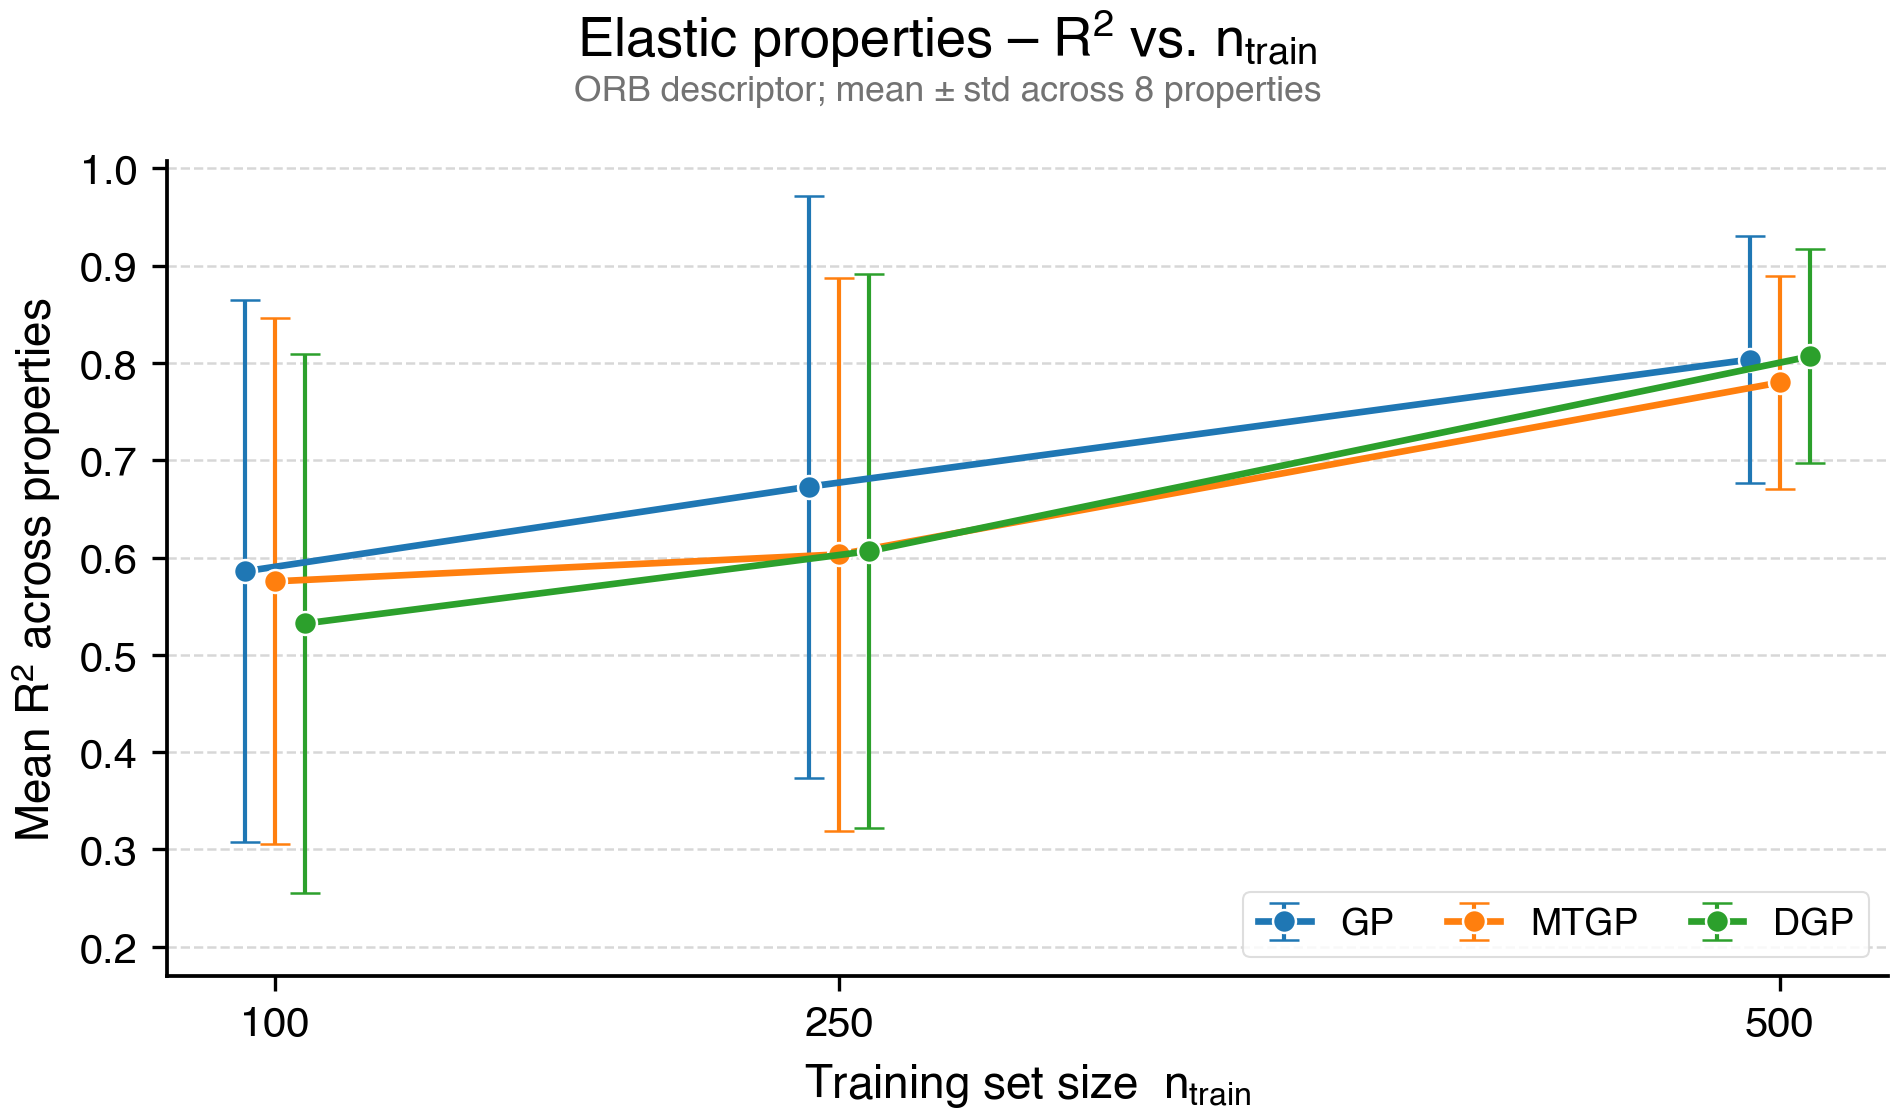
\includegraphics[width=\columnwidth]{figures/fig5_learning_curve_R2.png}
    \caption{Learning curves showing averaged \Rtwo{} as a function of training set size for all featuriser--surrogate combinations on the elastic tensor dataset. ORB\,+\,GP at $\ntrain = 100$ approaches the performance of SOAP\,+\,GP at $\ntrain = 500$.}
    \label{fig:learning_curves}
\end{figure}

\begin{table}[H]
    \centering
    \caption{Learning curve summary for ORB embeddings across all three surrogates on the elastic tensor dataset. \Rtwo{} values are averaged across all 8~elastic properties at the best PCA setting for each configuration.}
    \label{tab:learning_curves}
    \small
    \begin{tabular}{@{}lcccc@{}}
        \toprule
        \textbf{Surrogate} & $\ntrain{=}100$ & $\ntrain{=}250$ & $\ntrain{=}500$ & \textbf{Gain} \\
        \midrule
        GP  & 0.535 & 0.687 & 0.803 & +50\% \\
        MTGP & 0.530 & 0.627 & 0.780 & +47\% \\
        DGP  & 0.487 & 0.641 & 0.807 & +66\% \\
        \bottomrule
    \end{tabular}
\end{table}

ORB embeddings exhibit remarkable data efficiency.
At $\ntrain = 100$, ORB\,+\,GP already achieves $\bar{R}^2 \approx 0.535$ on the elastic tensor properties---surpassing SOAP\,+\,GP at $\ntrain = 500$ ($\bar{R}^2 = 0.445$).
The foundation model embeddings effectively provide a ``head start'' equivalent to $\sim$400 additional training samples.

The learning curves also reveal that the GP and DGP converge at different rates.
The GP shows the most consistent improvement from $\ntrain = 100$ to 500, gaining +50\% in \Rtwo{}.
The DGP shows the largest relative gain (+66\%) but starts lower at $\ntrain = 100$ due to insufficient data for variational training.
The MTGP shows the weakest scaling, plateauing earlier than the independent GP.
These results imply that in ultra-low-data campaigns ($\ntrain < 100$), the GP is the clear choice; the DGP requires at least $\sim$250 samples to match the GP.

\subsubsection{Dielectric and Phonon Learning Curves}
\label{sec:learning_curves_dielectric_phonon}

Learning curves for the dielectric and phonon datasets reveal markedly different scaling behaviour from the elastic case.
Figure~\ref{fig:learning_curves_dielectric} presents the averaged \Rtwo{} and Spearman correlation as a function of training set size for the dielectric constant dataset.
Unlike the elastic dataset, where all surrogates improve monotonically with data, the dielectric dataset shows that GP and MTGP \Rtwo{} values \emph{decrease} from $\ntrain = 100$ to $\ntrain = 500$, while the DGP remains relatively stable.
This counterintuitive behaviour reflects the heavy-tailed property distributions (polycrystalline dielectric constants span orders of magnitude): as the training set grows, it includes more extreme outliers that dominate the squared-error metric.
The Spearman correlations, by contrast, are stable or improve, confirming that the surrogates maintain their ranking capability even as absolute prediction degrades.

\begin{figure}[H]
    \centering
    \begin{subfigure}[t]{0.48\columnwidth}
        \centering
        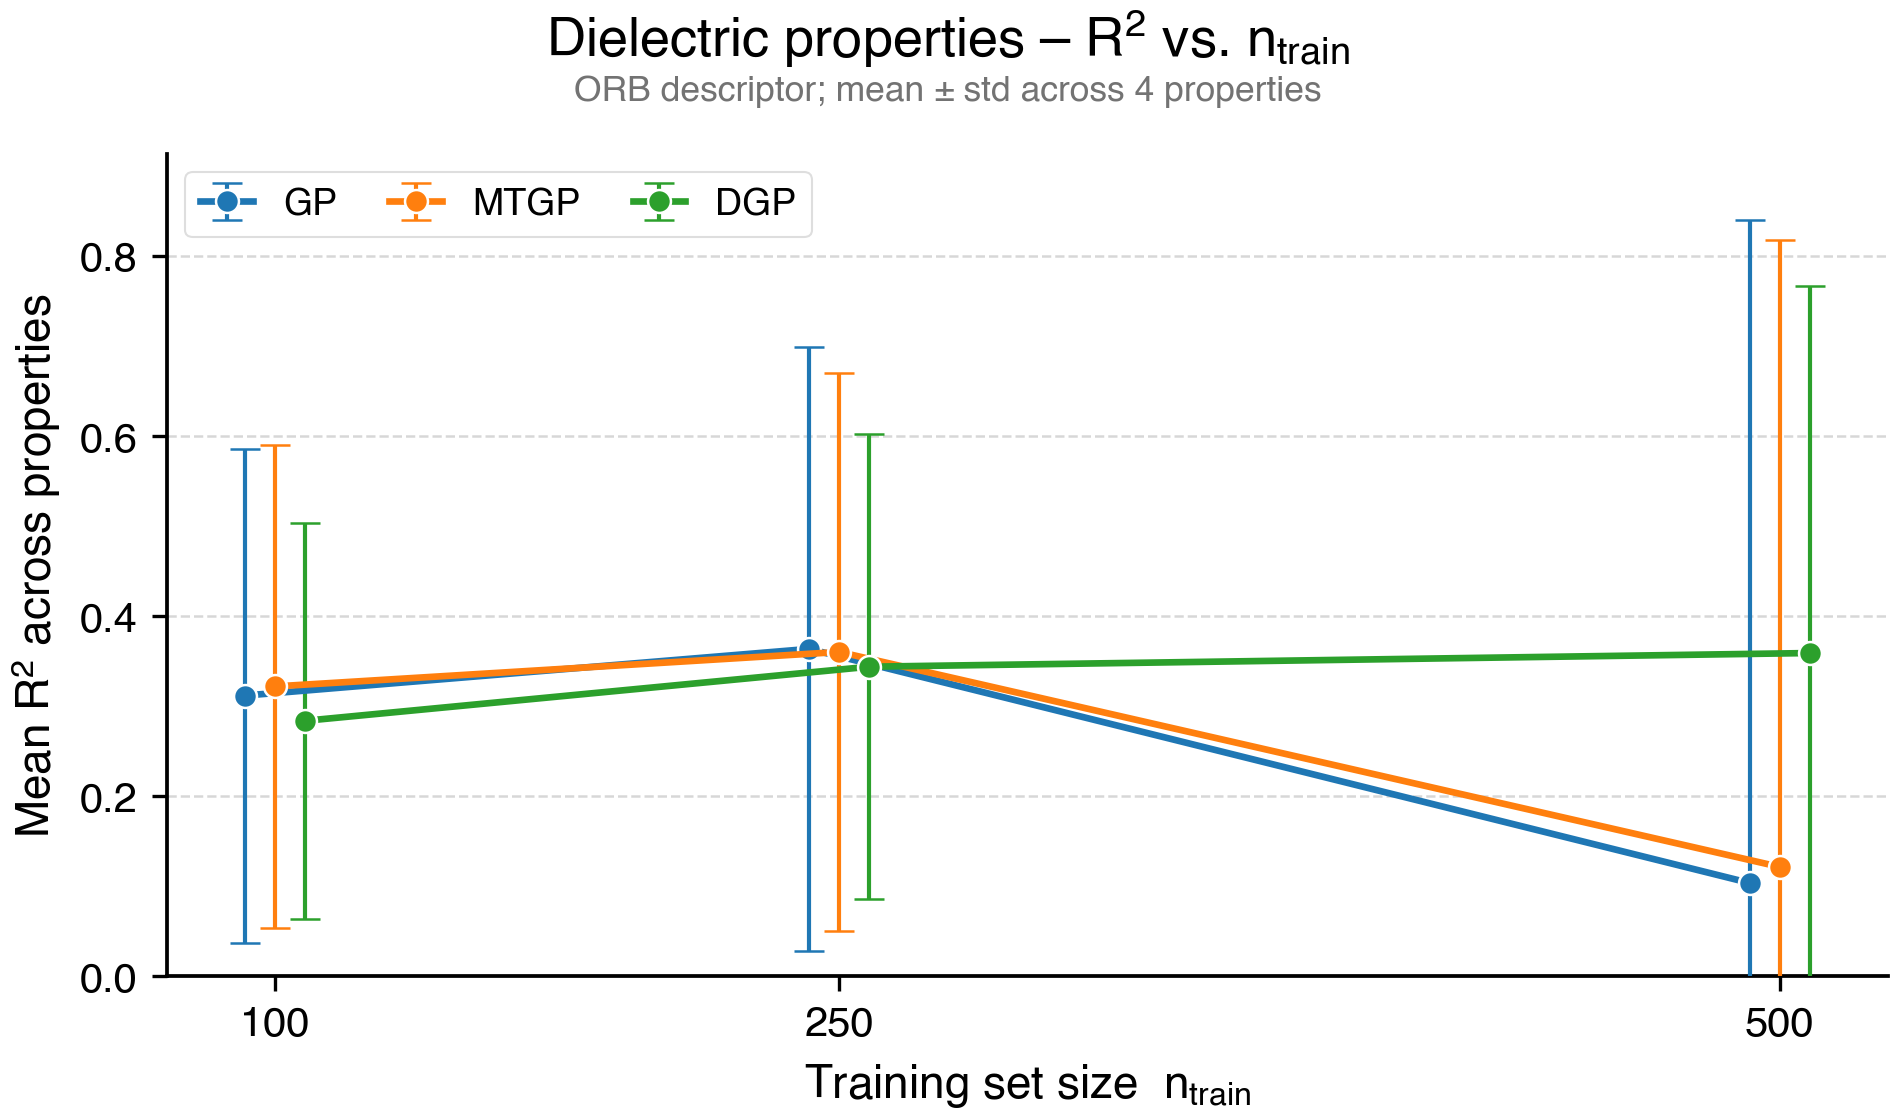
\includegraphics[width=\textwidth]{figures/fig_combined_dielectric_R2_learning_curve.png}
        \caption{Averaged \Rtwo{}}
        \label{fig:lc_dielectric_r2}
    \end{subfigure}
    \hfill
    \begin{subfigure}[t]{0.48\columnwidth}
        \centering
        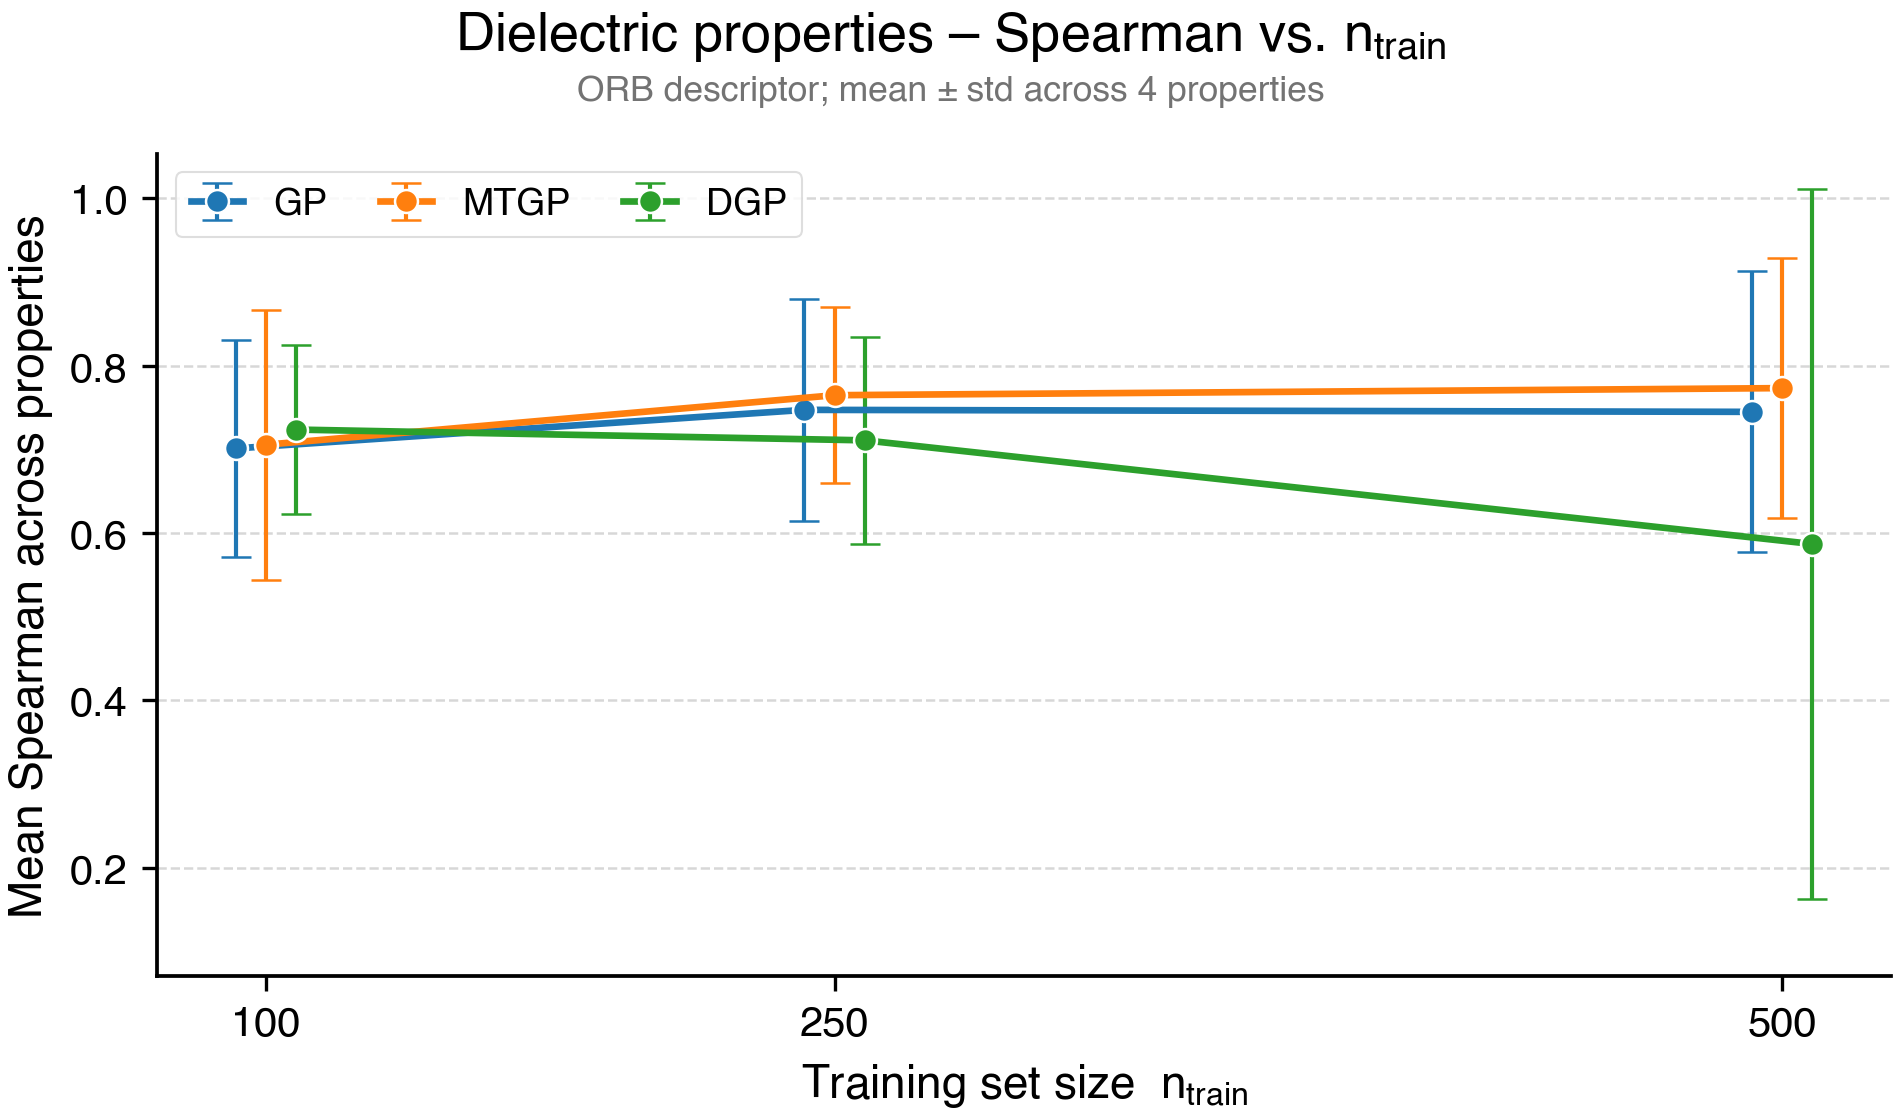
\includegraphics[width=\textwidth]{figures/fig_combined_dielectric_Spearman_learning_curve.png}
        \caption{Averaged Spearman $\rho$}
        \label{fig:lc_dielectric_spearman}
    \end{subfigure}
    \caption{Learning curves for the dielectric constant dataset (ORB descriptor, best PCA per surrogate). GP and MTGP \Rtwo{} values decrease with training size due to heavy-tailed property distributions, while Spearman correlations remain stable, reinforcing the finding that ranking accuracy is more robust than regression accuracy for electronically complex properties.}
    \label{fig:learning_curves_dielectric}
\end{figure}

Figure~\ref{fig:learning_curves_phonon} shows the analogous learning curves for the phonon dielectric dataset.
Here, all three surrogates show modest improvement with training size, and the DGP achieves the best \Rtwo{} at $\ntrain = 500$---consistent with its ability to model non-linear structure--property relationships given sufficient data.
The large error bars on the DGP reflect its sensitivity to the random initialisation of variational parameters, a practical consideration for reproducibility.
Spearman correlations for the phonon dataset improve steadily, with MTGP achieving the highest ranking accuracy at $\ntrain = 500$, consistent with the multi-task signal from correlated dielectric properties.

\begin{figure}[H]
    \centering
    \begin{subfigure}[t]{0.48\columnwidth}
        \centering
        
\includegraphics[width=\textwidth]{figures/fig_combined_phonon_R2_learning_curve.png}
        \caption{Averaged \Rtwo{}}
        \label{fig:lc_phonon_r2}
    \end{subfigure}
    \hfill
    \begin{subfigure}[t]{0.48\columnwidth}
        \centering
        
\includegraphics[width=\textwidth]{figures/fig_combined_phonon_Spearman_learning_curve.png}
        \caption{Averaged Spearman $\rho$}
        \label{fig:lc_phonon_spearman}
    \end{subfigure}
    \caption{Learning curves for the phonon dielectric dataset (ORB descriptor, best PCA per surrogate). All surrogates show modest improvement with training size. DGP achieves the best \Rtwo{} at $\ntrain = 500$ but with large variance. MTGP shows the strongest Spearman scaling, reaching $\bar{\rho} > 0.83$ at $\ntrain = 500$.}
    \label{fig:learning_curves_phonon}
\end{figure}

The contrasting learning curve behaviours across the three datasets reveal a key insight: the standard ``more data always helps'' intuition holds for geometric properties (elastic) and vibrational properties (phonon), but breaks down for electronic properties (dielectric) when measured by \Rtwo{}.
This dataset-dependent scaling further supports our recommendation to use Spearman correlation as the primary evaluation metric for surrogates targeting Bayesian optimisation.

\FloatBarrier
\subsection{Per-Property Difficulty Analysis}
\label{sec:property_analysis}

Not all properties are created equal.
Figure~\ref{fig:difficulty_all} presents property difficulty matrices for all three datasets, and the radar charts in Figure~\ref{fig:radar_all} visualise ORB's per-property profile.

\begin{figure*}[!htb]
    \centering
    \begin{subfigure}[t]{0.32\textwidth}
        \centering
        
\includegraphics[width=\textwidth]{figures/fig6_property_difficulty.pdf}
        \caption{Elastic tensor}
        \label{fig:diff_elastic}
    \end{subfigure}
    \hfill
    \begin{subfigure}[t]{0.32\textwidth}
        \centering
        
\includegraphics[width=\textwidth]{figures/fig_difficulty_dielectric_n500.pdf}
        \caption{Dielectric constant}
        \label{fig:diff_dielectric}
    \end{subfigure}
    \hfill
    \begin{subfigure}[t]{0.32\textwidth}
        \centering
        
\includegraphics[width=\textwidth]{figures/fig_difficulty_phonon_n500.pdf}
        \caption{Phonon dielectric}
        \label{fig:diff_phonon}
    \end{subfigure}
    \caption{Property difficulty matrices showing the best-achievable \Rtwo{} per property across all featuriser--PCA combinations at $\ntrain = 500$, broken down by surrogate model. (a)~Elastic: bulk modulus variants are easiest; anisotropy and Poisson's ratio are hardest. (b)~Dielectric: band gap is easiest; polycrystalline dielectric constants are hardest. (c)~Phonon: last phonon DOS peak is well predicted; dielectric constants are essentially unpredictable.}
    \label{fig:difficulty_all}
\end{figure*}

\begin{figure*}[!htb]
    \centering
    \begin{subfigure}[t]{0.32\textwidth}
        \centering
        
\includegraphics[width=\textwidth]{figures/fig7_radar_orb_R2.pdf}
        \caption{Elastic tensor}
        \label{fig:radar_elastic}
    \end{subfigure}
    \hfill
    \begin{subfigure}[t]{0.32\textwidth}
        \centering
        
\includegraphics[width=\textwidth]{figures/fig_radar_dielectric_orb_R2_n500.pdf}
        \caption{Dielectric constant}
        \label{fig:radar_dielectric}
    \end{subfigure}
    \hfill
    \begin{subfigure}[t]{0.32\textwidth}
        \centering
        
\includegraphics[width=\textwidth]{figures/fig_radar_phonon_orb_R2_n500.pdf}
        \caption{Phonon dielectric}
        \label{fig:radar_phonon}
    \end{subfigure}
    \caption{Radar charts showing ORB's per-property \Rtwo{} across GP, MTGP, and DGP at $\ntrain = 500$ for each dataset. The elastic dataset shows the most uniform performance across properties; the dielectric and phonon datasets exhibit extreme asymmetry between easy and hard properties.}
    \label{fig:radar_all}
\end{figure*}

\textbf{Elastic tensor.}
Table~\ref{tab:property_difficulty_elastic} ranks each property by best achievable \Rtwo{}.
Bulk modulus properties ($K$) are the easiest to predict, with $R^2 > 0.91$ for all three variants (Voigt, VRH, Reuss).
This is physically intuitive: bulk modulus is primarily determined by bond stiffness and local atomic chemistry---precisely the information most directly encoded in structural embeddings.
The Voigt average (uniform strain) is the easiest ($R^2 = 0.931$), while the Reuss average (uniform stress) is slightly harder ($R^2 = 0.911$), consistent with the Reuss bound's greater sensitivity to microstructural heterogeneity.
Shear modulus ($G$) properties occupy the middle ground ($R^2 = 0.78$--$0.83$).
Elastic anisotropy ($R^2 = 0.746$) and Poisson's ratio ($R^2 = 0.658$) are the most challenging.
Notably, elastic anisotropy is the one property where the DGP clearly outperforms the GP ($R^2 = 0.746$ vs.\ 0.582), suggesting that its non-linear feature transformations are beneficial for properties with complex structure--property relationships.

\begin{table}[H]
    \centering
    \caption{Property difficulty ranking on the elastic tensor dataset ($\ntrain = 500$). Each row reports the best \Rtwo{} achieved across all featuriser and PCA combinations.}
    \label{tab:property_difficulty_elastic}
    \small
    \begin{tabular}{@{}lllcc@{}}
        \toprule
        \textbf{Property} & \textbf{Best Feat.} & \textbf{Surr.} & \textbf{PCA} & \textbf{\Rtwo{}} \\
        \midrule
        $K_{\text{Voigt}}$   & ORB & GP  & 50 & 0.931 \\
        $K_{\text{VRH}}$     & ORB & GP  & 50 & 0.922 \\
        $K_{\text{Reuss}}$   & ORB & GP  & 50 & 0.911 \\
        $G_{\text{Voigt}}$   & ORB & GP  & 50 & 0.832 \\
        $G_{\text{VRH}}$     & ORB & GP  & 50 & 0.812 \\
        $G_{\text{Reuss}}$   & ORB & GP  & 50 & 0.781 \\
        Elastic aniso.       & ORB & DGP & 25 & 0.746 \\
        Poisson's ratio      & ORB & GP  & 50 & 0.658 \\
        \bottomrule
    \end{tabular}
\end{table}

\textbf{Dielectric constant.}
The dielectric dataset reveals a sharp split between properties (Table~\ref{tab:property_difficulty_dielectric}).
Band gap is the easiest property ($R^2 = 0.852$, ORB\,+\,GP, PCA\,=\,50), reflecting its strong correlation with local bonding chemistry.
Refractive index ($n$) achieves moderate \Rtwo{} values ($R^2 = 0.552$, DGP\,+\,ORB, PCA\,=\,10), while the polycrystalline dielectric constants are essentially unpredictable ($R^2 < 0$ for poly\_electronic; $R^2 \approx 0.09$ for poly\_total at best).
The negative \Rtwo{} values for poly\_electronic across all featurisers indicate that no geometric embedding---classical or foundation-model-based---captures the electronic polarisability information needed for this property.

\begin{table}[H]
    \centering
    \caption{Property difficulty ranking on the dielectric constant dataset ($\ntrain = 500$).}
    \label{tab:property_difficulty_dielectric}
    \small
    \begin{tabular}{@{}lllcc@{}}
        \toprule
        \textbf{Property} & \textbf{Best Feat.} & \textbf{Surr.} & \textbf{PCA} & \textbf{\Rtwo{}} \\
        \midrule
        band\_gap        & ORB  & GP   & 50 & 0.852 \\
        $n$              & ORB  & DGP  & 10 & 0.552 \\
        poly\_total      & UMA  & DGP  & 25 & 0.111 \\
        poly\_electronic & MACE & DGP  & 25 & $-$0.180 \\
        \bottomrule
    \end{tabular}
\end{table}

\textbf{Phonon dielectric.}
The phonon dataset shows the most extreme property asymmetry (Table~\ref{tab:property_difficulty_phonon}).
The last phonon DOS peak is well predicted by all methods, with ORB\,+\,GP achieving $R^2 = 0.911$.
This is physically sensible: the highest-frequency phonon mode is strongly determined by the lightest atoms and their bond stiffness---information directly accessible from the crystal structure.
In contrast, both dielectric constants (eps\_electronic and eps\_total) yield $R^2 \approx -0.001$ for \emph{every} featuriser and surrogate.
The near-zero \Rtwo{} coupled with high Spearman correlations ($\rho = 0.930$ for eps\_electronic with ORB\,+\,GP) reveals that the surrogates correctly rank materials but fail to predict absolute values, likely due to outlier structures with extreme dielectric constants dominating the RMSE.

\begin{table}[H]
    \centering
    \caption{Property difficulty ranking on the phonon dielectric dataset ($\ntrain = 500$). Despite $R^2 \approx -0.001$ for dielectric properties, the high Spearman correlations indicate useful ranking capability.}
    \label{tab:property_difficulty_phonon}
    \small
    \begin{tabular}{@{}lllccc@{}}
        \toprule
        \textbf{Property} & \textbf{Best Feat.} & \textbf{Surr.} & \textbf{PCA} & \textbf{\Rtwo{}} & \textbf{$\rho$} \\
        \midrule
        last\_phdos\_peak  & ORB  & GP   & 50 & 0.911 & 0.947 \\
        eps\_electronic    & ORB  & GP   & 50 & $-$0.001 & 0.930 \\
        eps\_total         & ORB  & MTGP & 10 & $-$0.001 & 0.658 \\
        \bottomrule
    \end{tabular}
\end{table}


\subsection{Parity Plots and the R$^{2}$--Spearman Gap}
\label{sec:parity_plots}

Section~\ref{sec:property_analysis} reported R$^{2}$ and $\rho$ per property; Figure~\ref{fig:metric_disagreement} plots them against each other for all 16 (dataset, property) pairs at our recommended setting (ORB\,+\,GP, PCA\,=\,50, $\ntrain = 500$).
Most properties cluster near the $\rho = R^{2}$ diagonal where both metrics agree.
Six sit well above it.
The two extremes are eps\_electronic ($R^{2} \approx 0$, $\rho = 0.93$) and poly\_electronic ($R^{2} = -0.87$, $\rho = 0.69$): the heavier the property's tail, the more the two metrics disagree.
We return to this in Section~\ref{sec:spearman_r2}.

\begin{figure}[H]
    \centering
    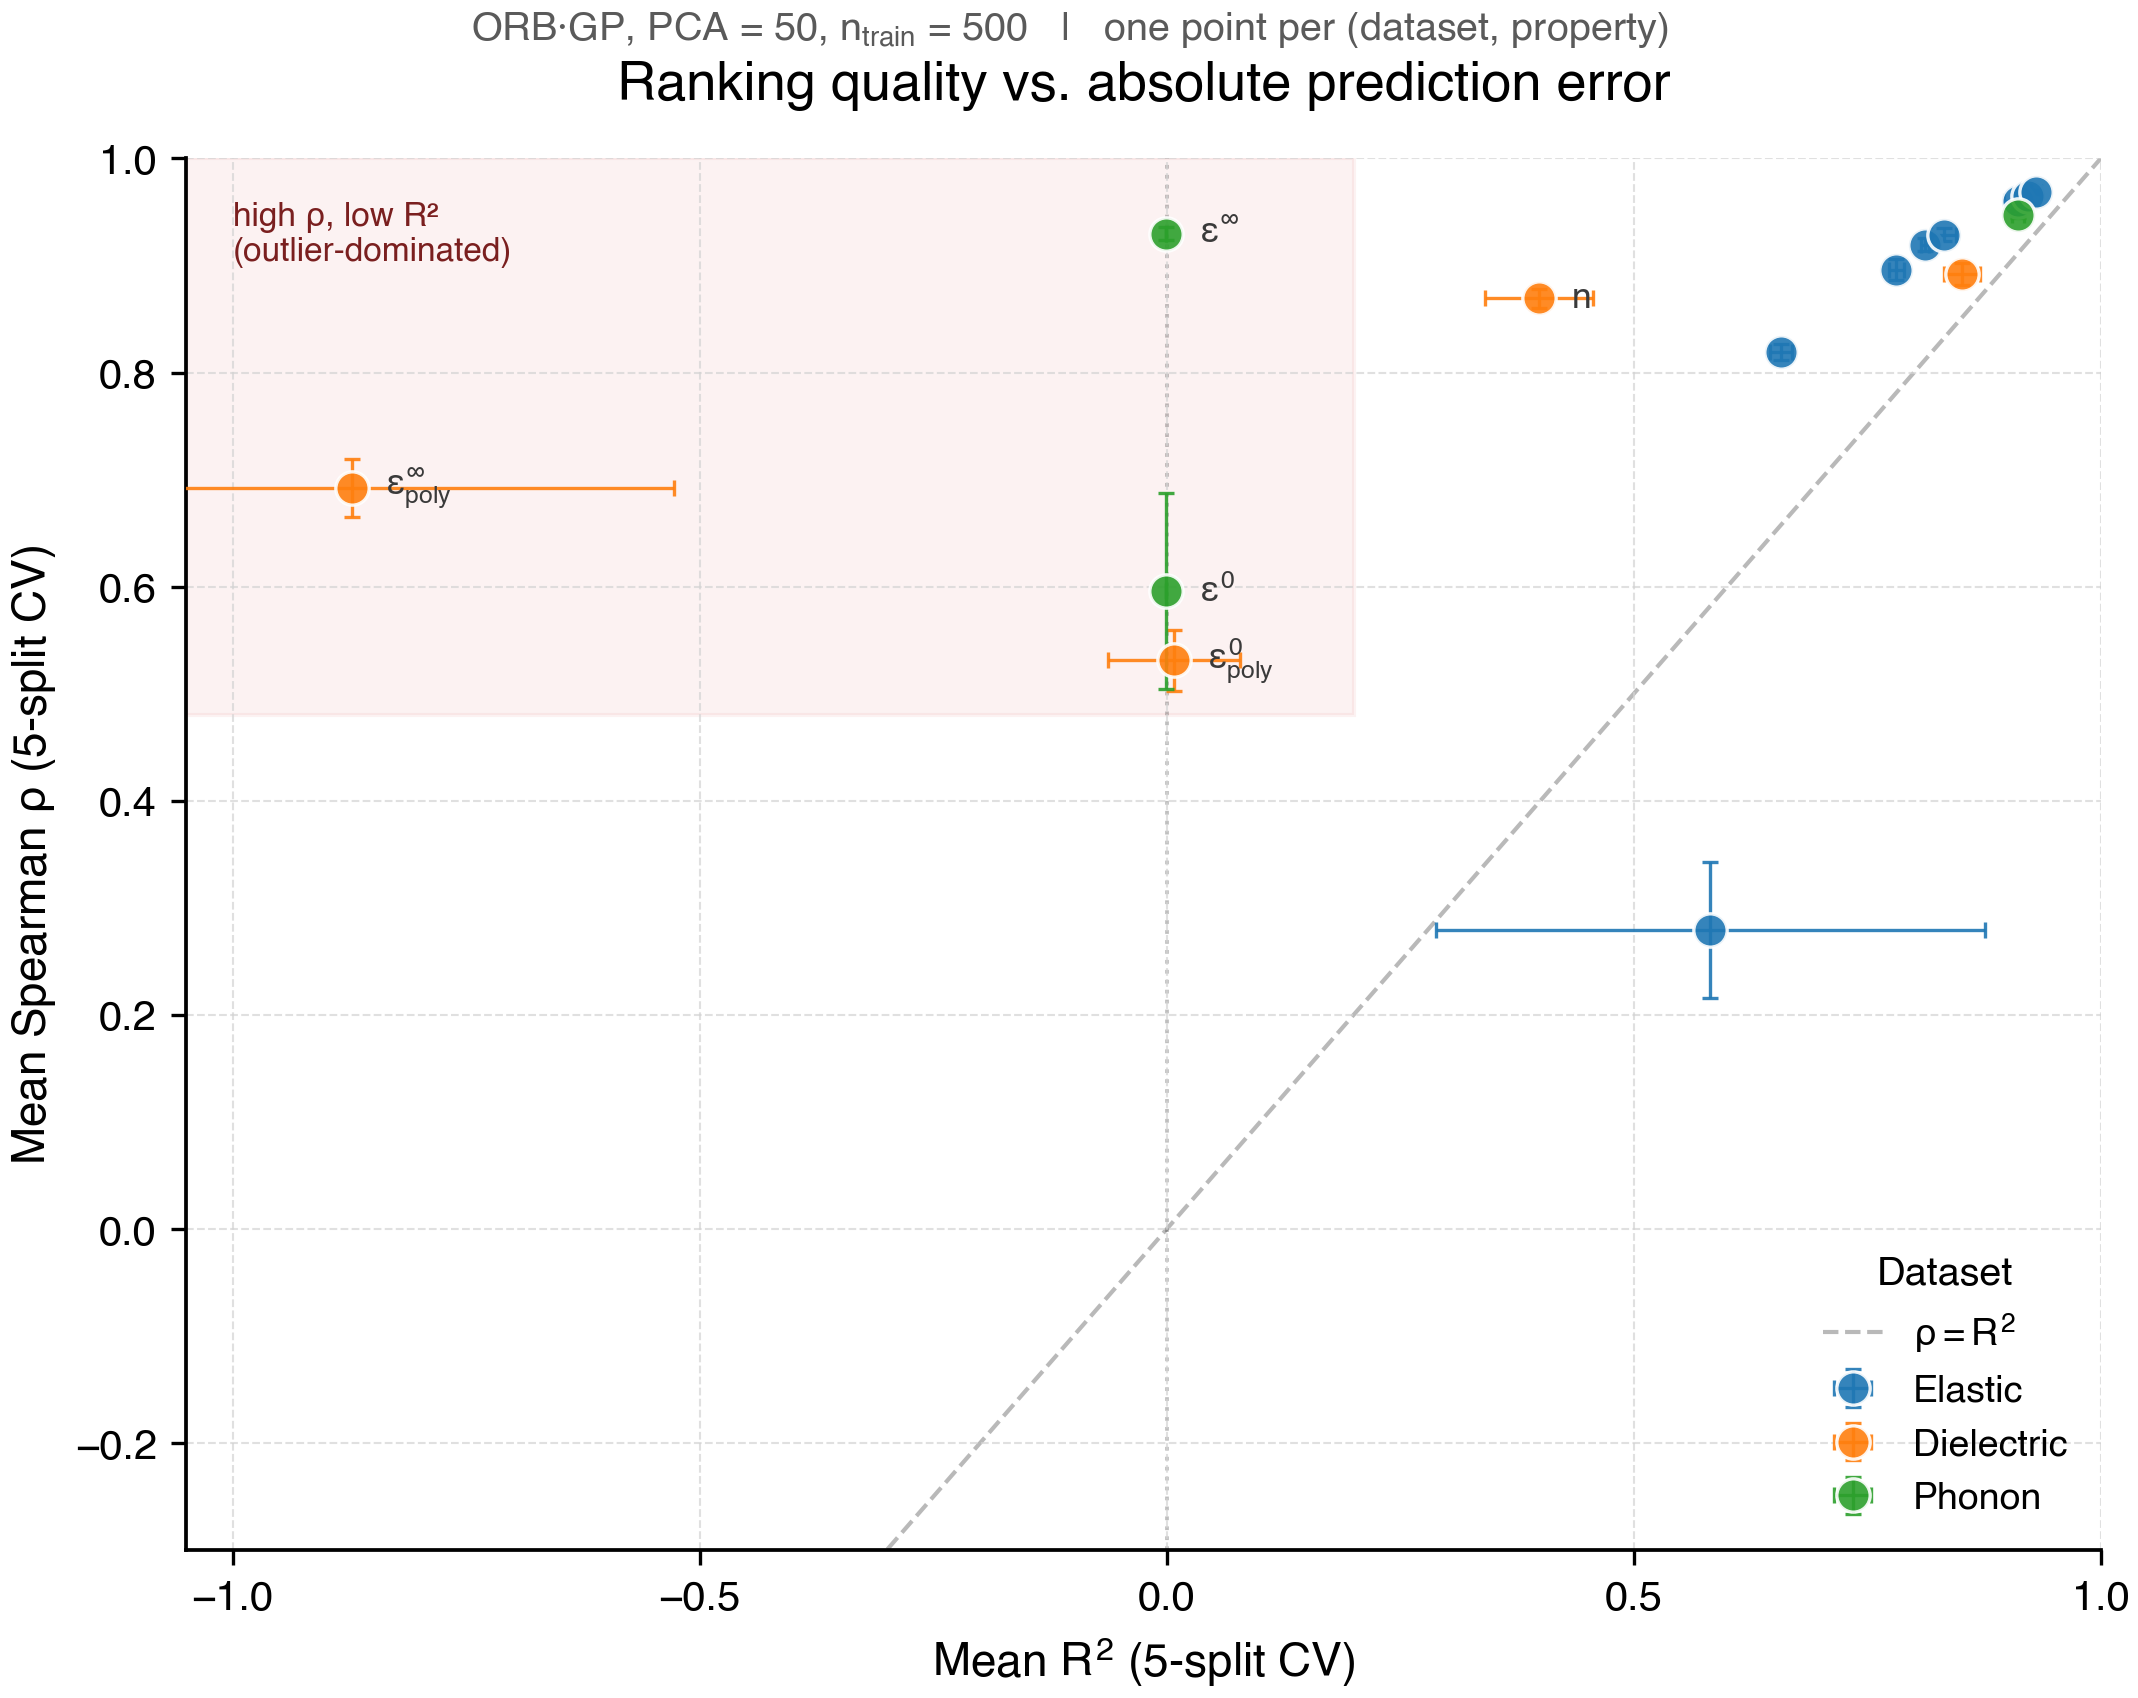
\includegraphics[width=\columnwidth]{figures/fig_metric_disagreement.png}
    \caption{Mean Spearman~$\rho$ vs.\ mean \Rtwo{} across all 16 (dataset, property) pairs under ORB\,+\,GP, PCA\,=\,50, $\ntrain = 500$, with 5-split standard-deviation bars. Points on the dashed $\rho = R^{2}$ diagonal indicate metric agreement. The shaded zone marks the regime where rank correlation remains high while \Rtwo{} collapses---driven by extreme outliers in the property distribution. Properties with $R^{2} < 0.3$ are labelled.}
    \label{fig:metric_disagreement}
\end{figure}

\FloatBarrier
Figure~\ref{fig:parity_examples} shows the best-predicted property in each dataset under the same setting (split~1).
All three sit tightly on the diagonal with calibrated uncertainty bands.
We do not show parity for the harder properties because their absolute-scale outliers dominate the visual; their cross-property structure is what Figure~\ref{fig:metric_disagreement} captures.

\begin{figure*}[!htb]
    \centering
    \begin{subfigure}[t]{0.32\textwidth}
        \centering
        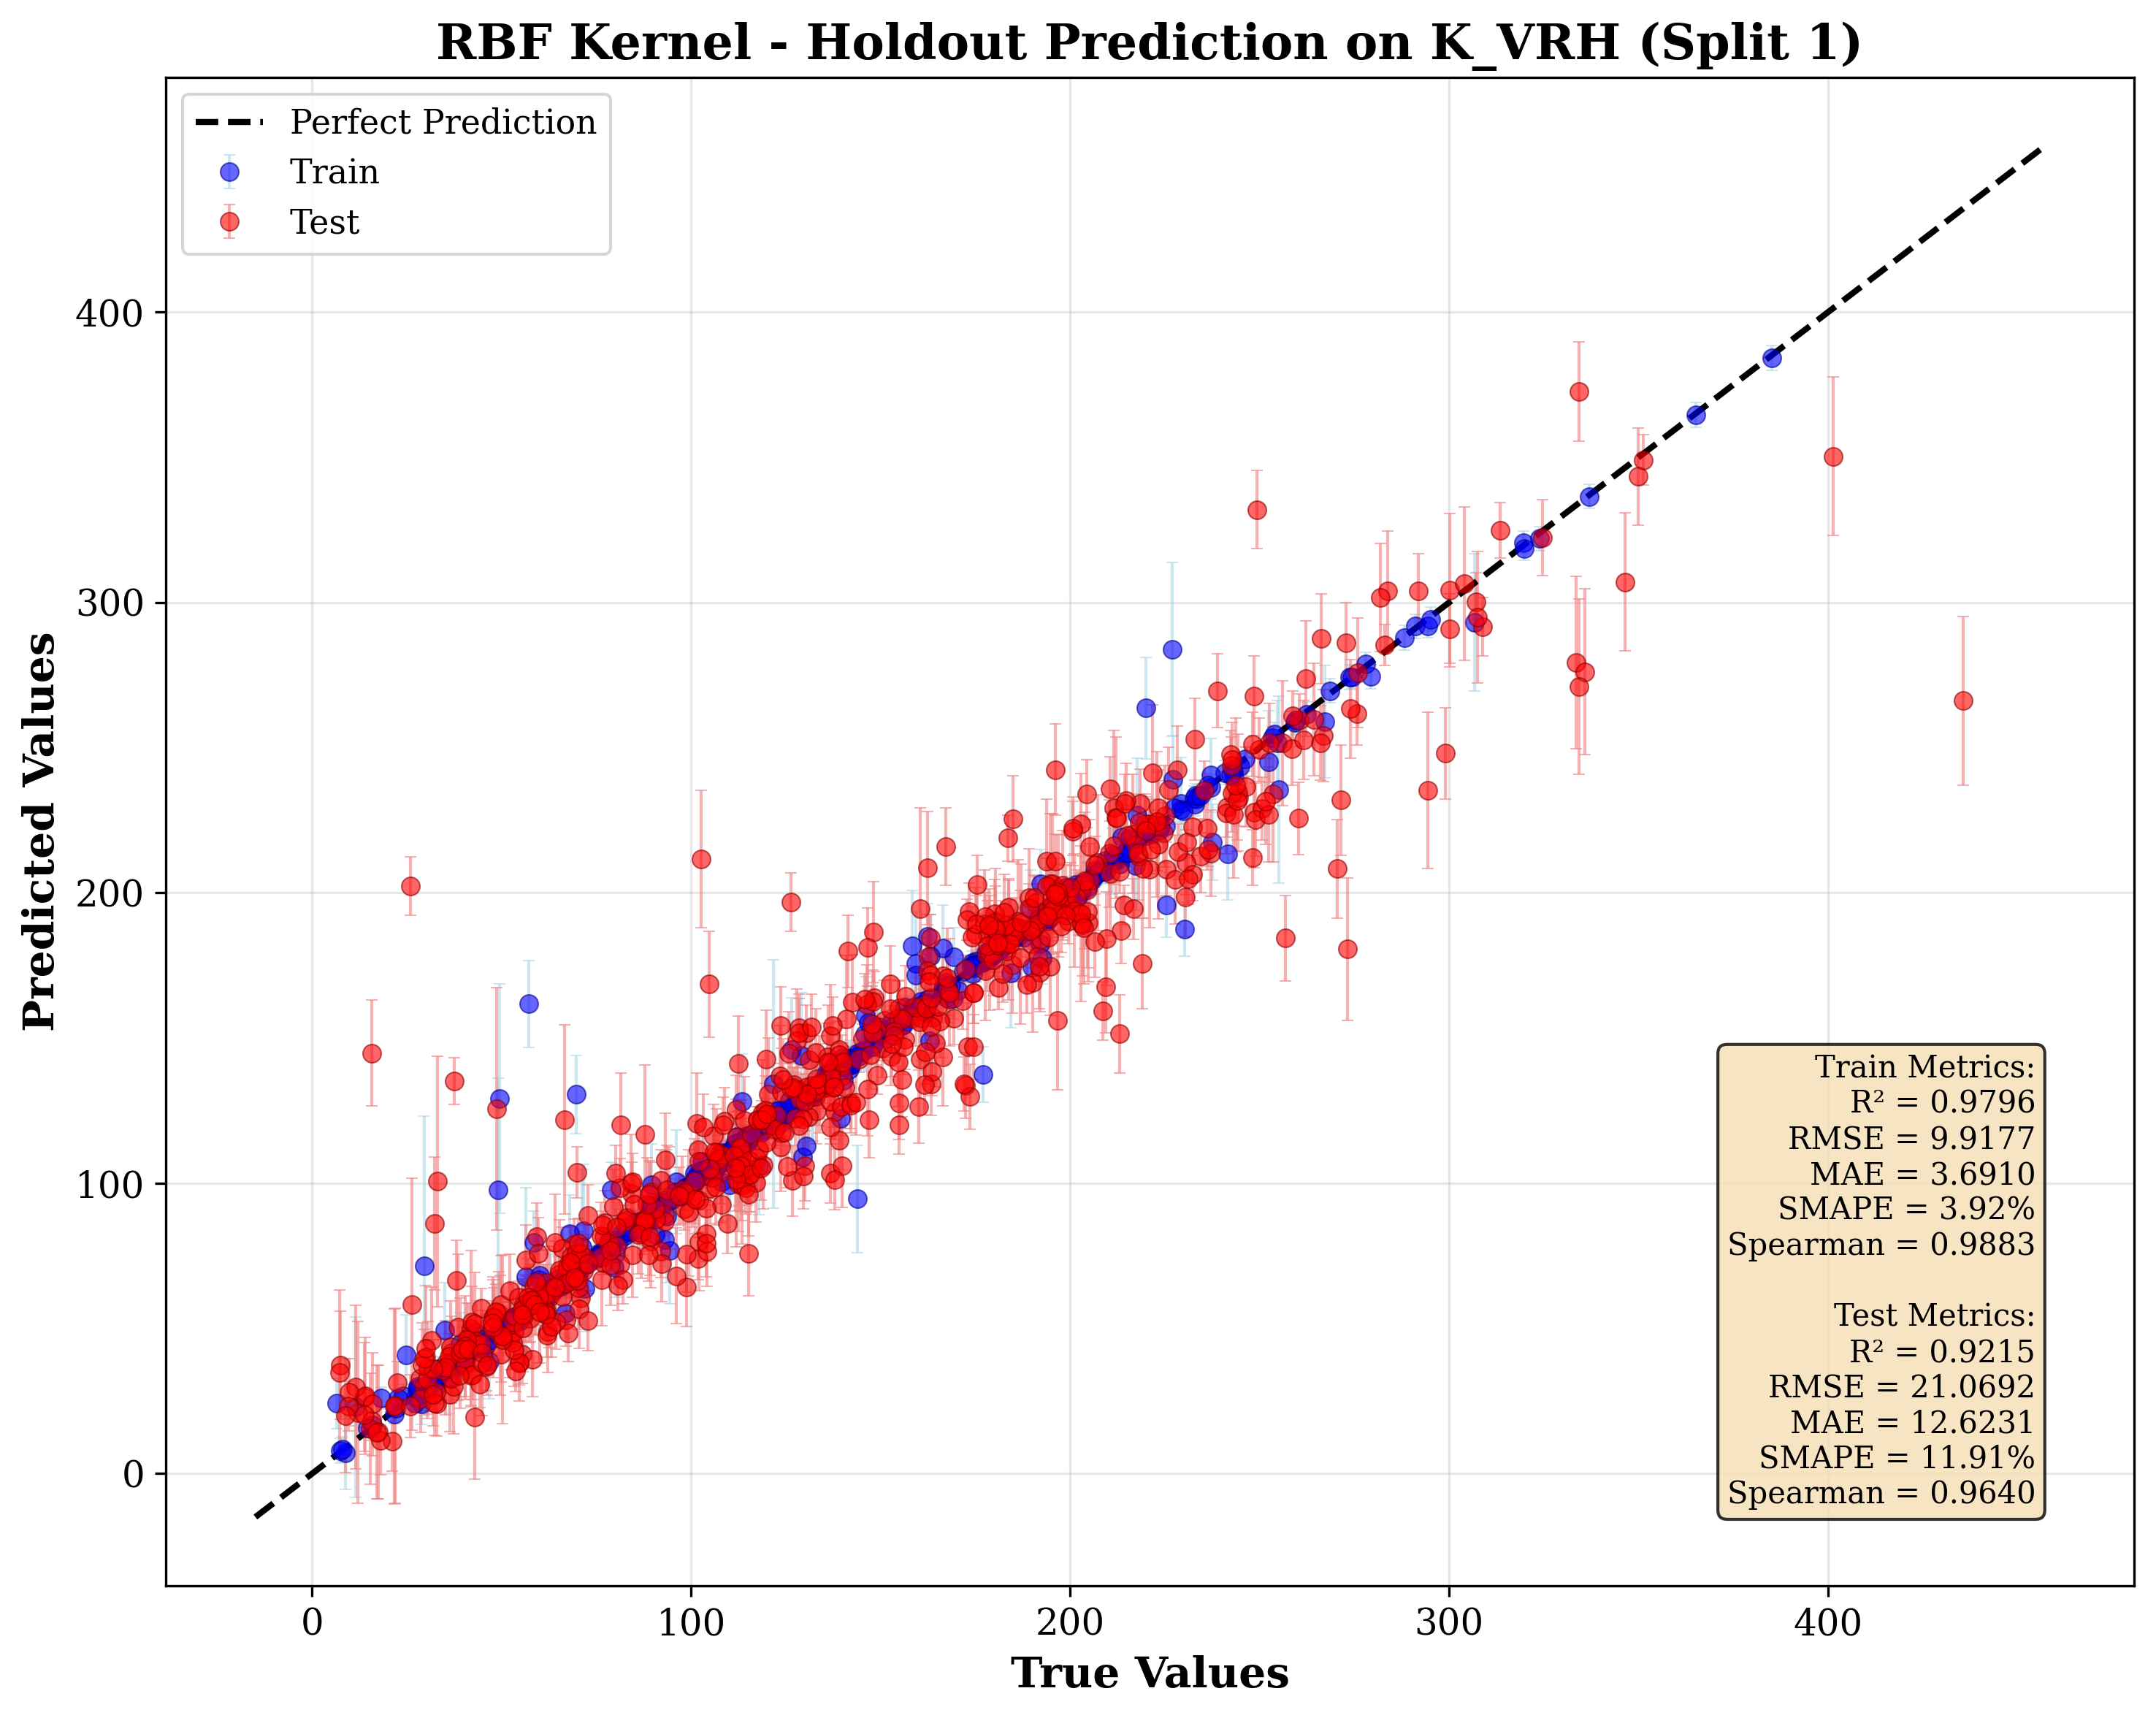
\includegraphics[width=\textwidth]{figures/fig_parity_elastic_K_VRH_orb_gp.png}
        \caption{Elastic: $K_{\text{VRH}}$ ($R^{2} = 0.922$)}
    \end{subfigure}
    \hfill
    \begin{subfigure}[t]{0.32\textwidth}
        \centering
        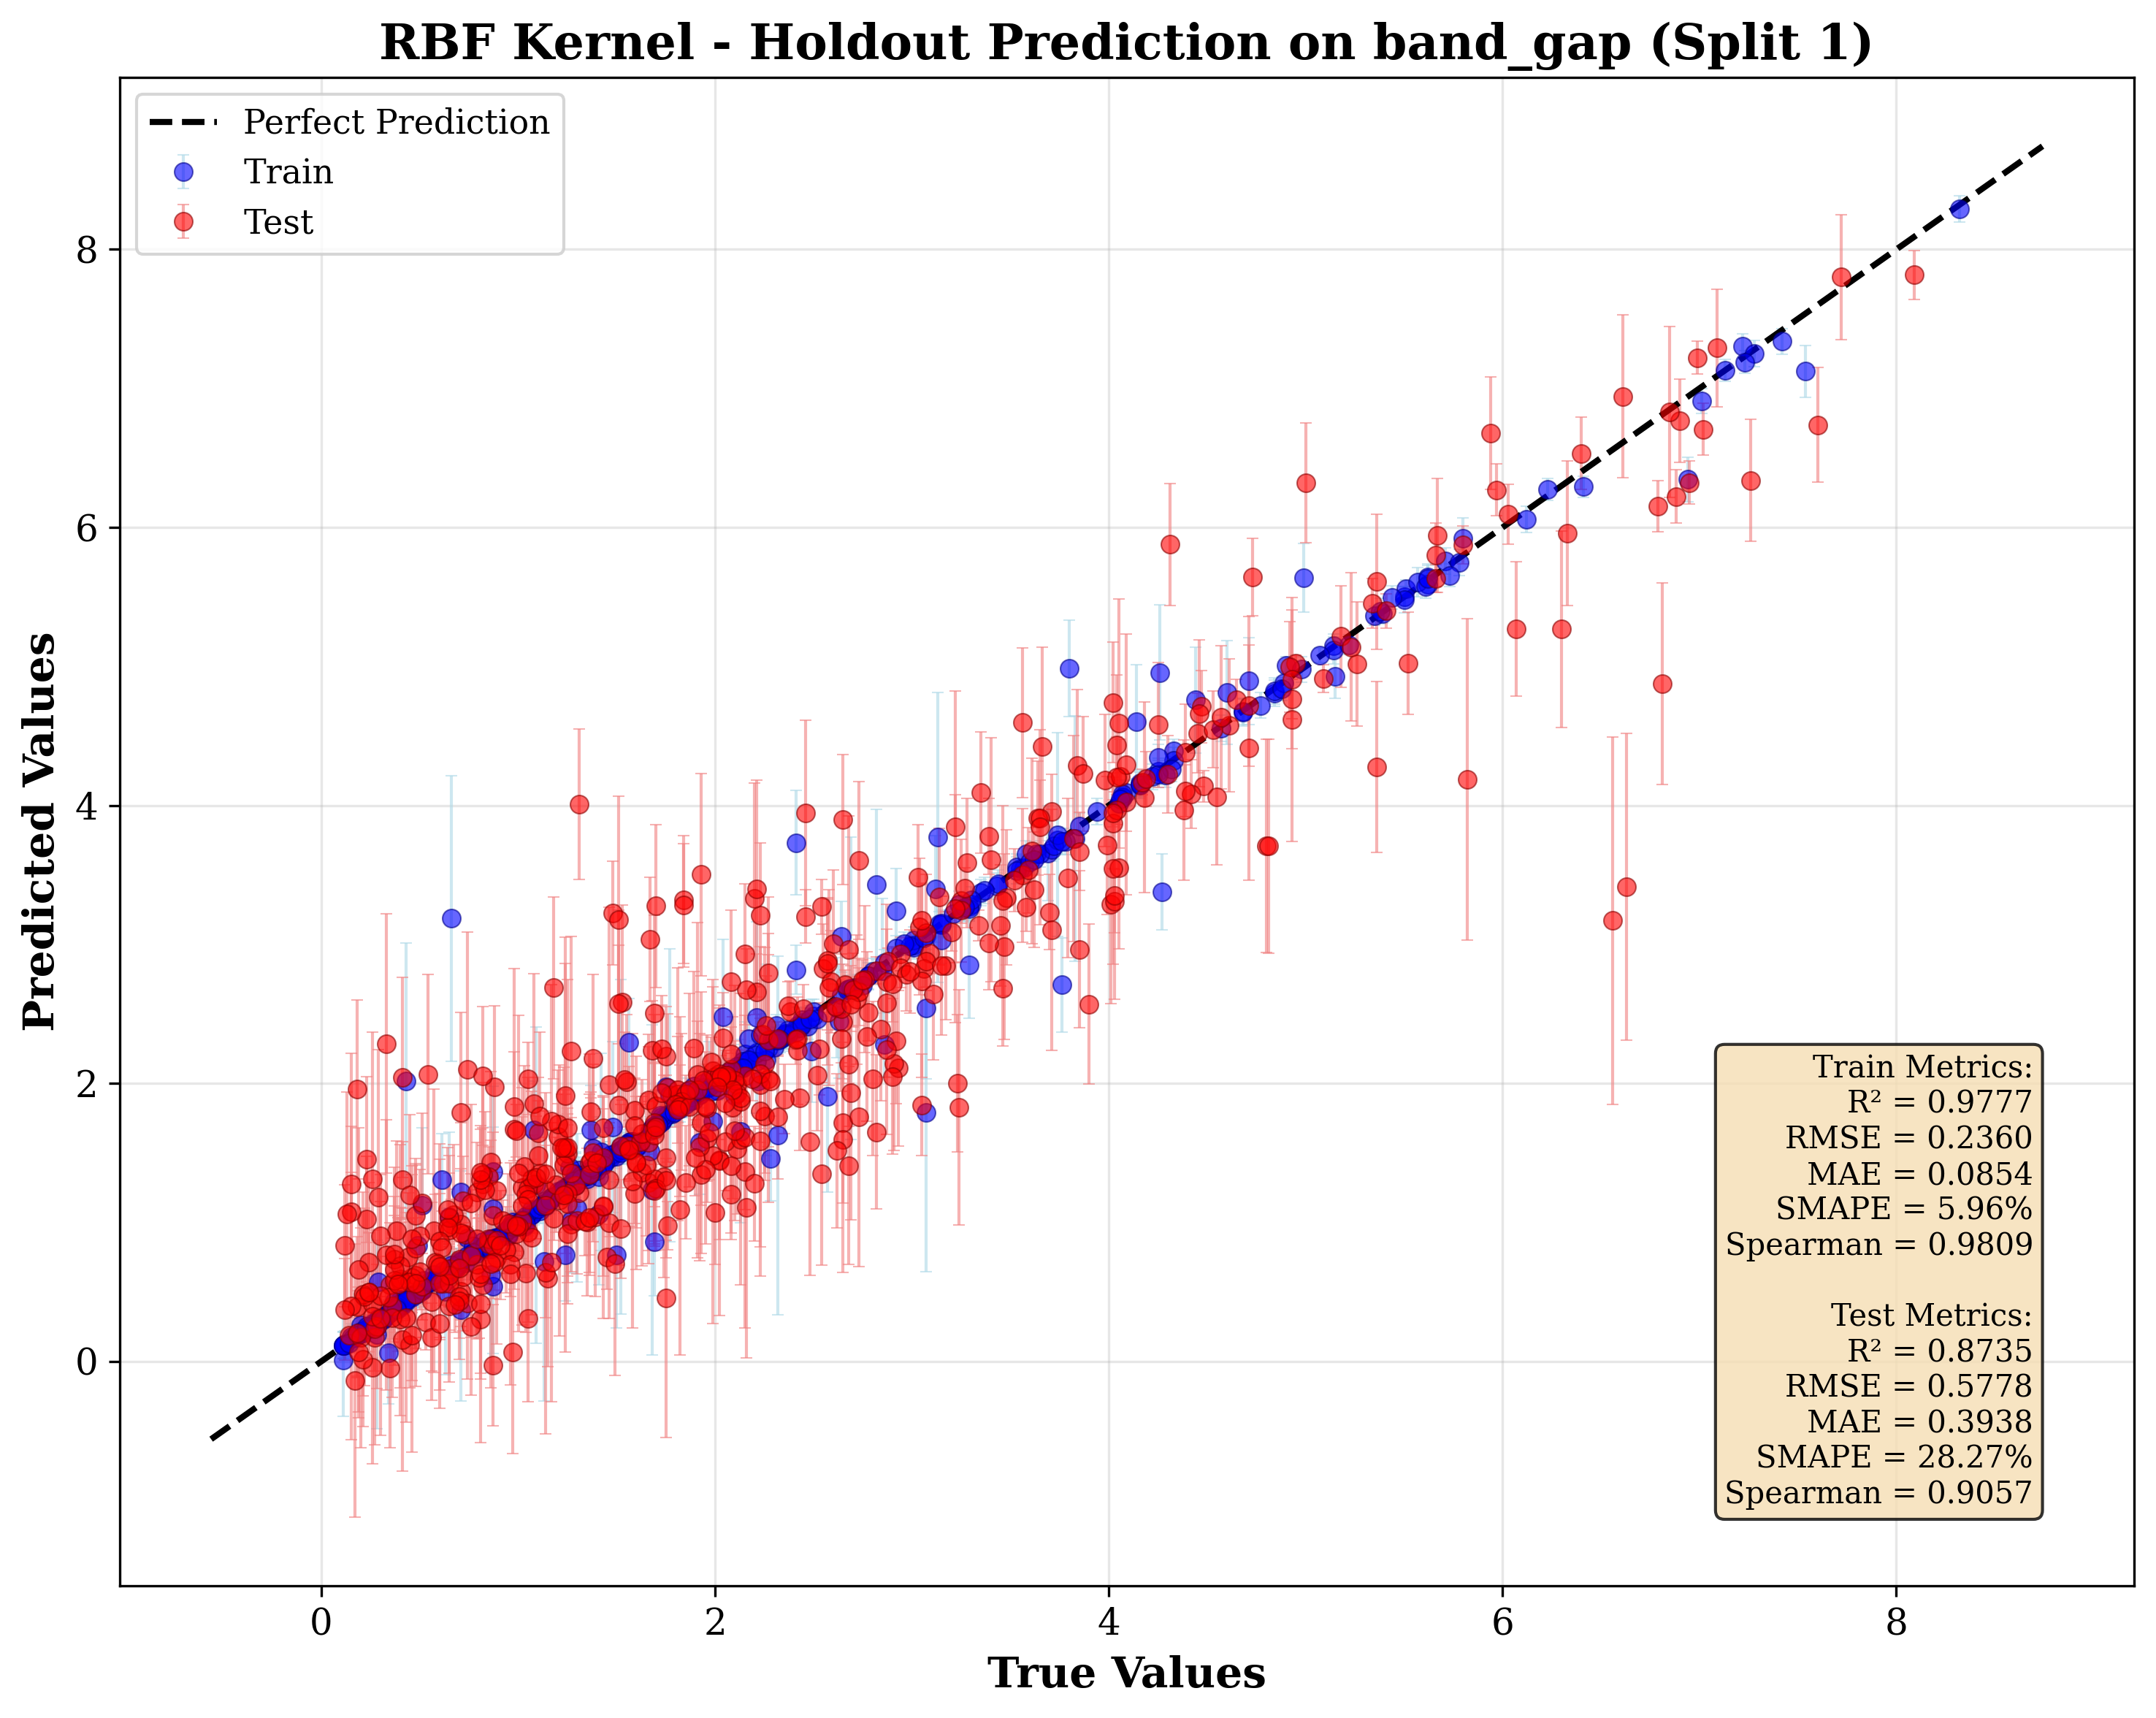
\includegraphics[width=\textwidth]{figures/fig_parity_dielectric_band_gap_orb_gp.png}
        \caption{Dielectric: band gap ($R^{2} = 0.852$)}
    \end{subfigure}
    \hfill
    \begin{subfigure}[t]{0.32\textwidth}
        \centering
        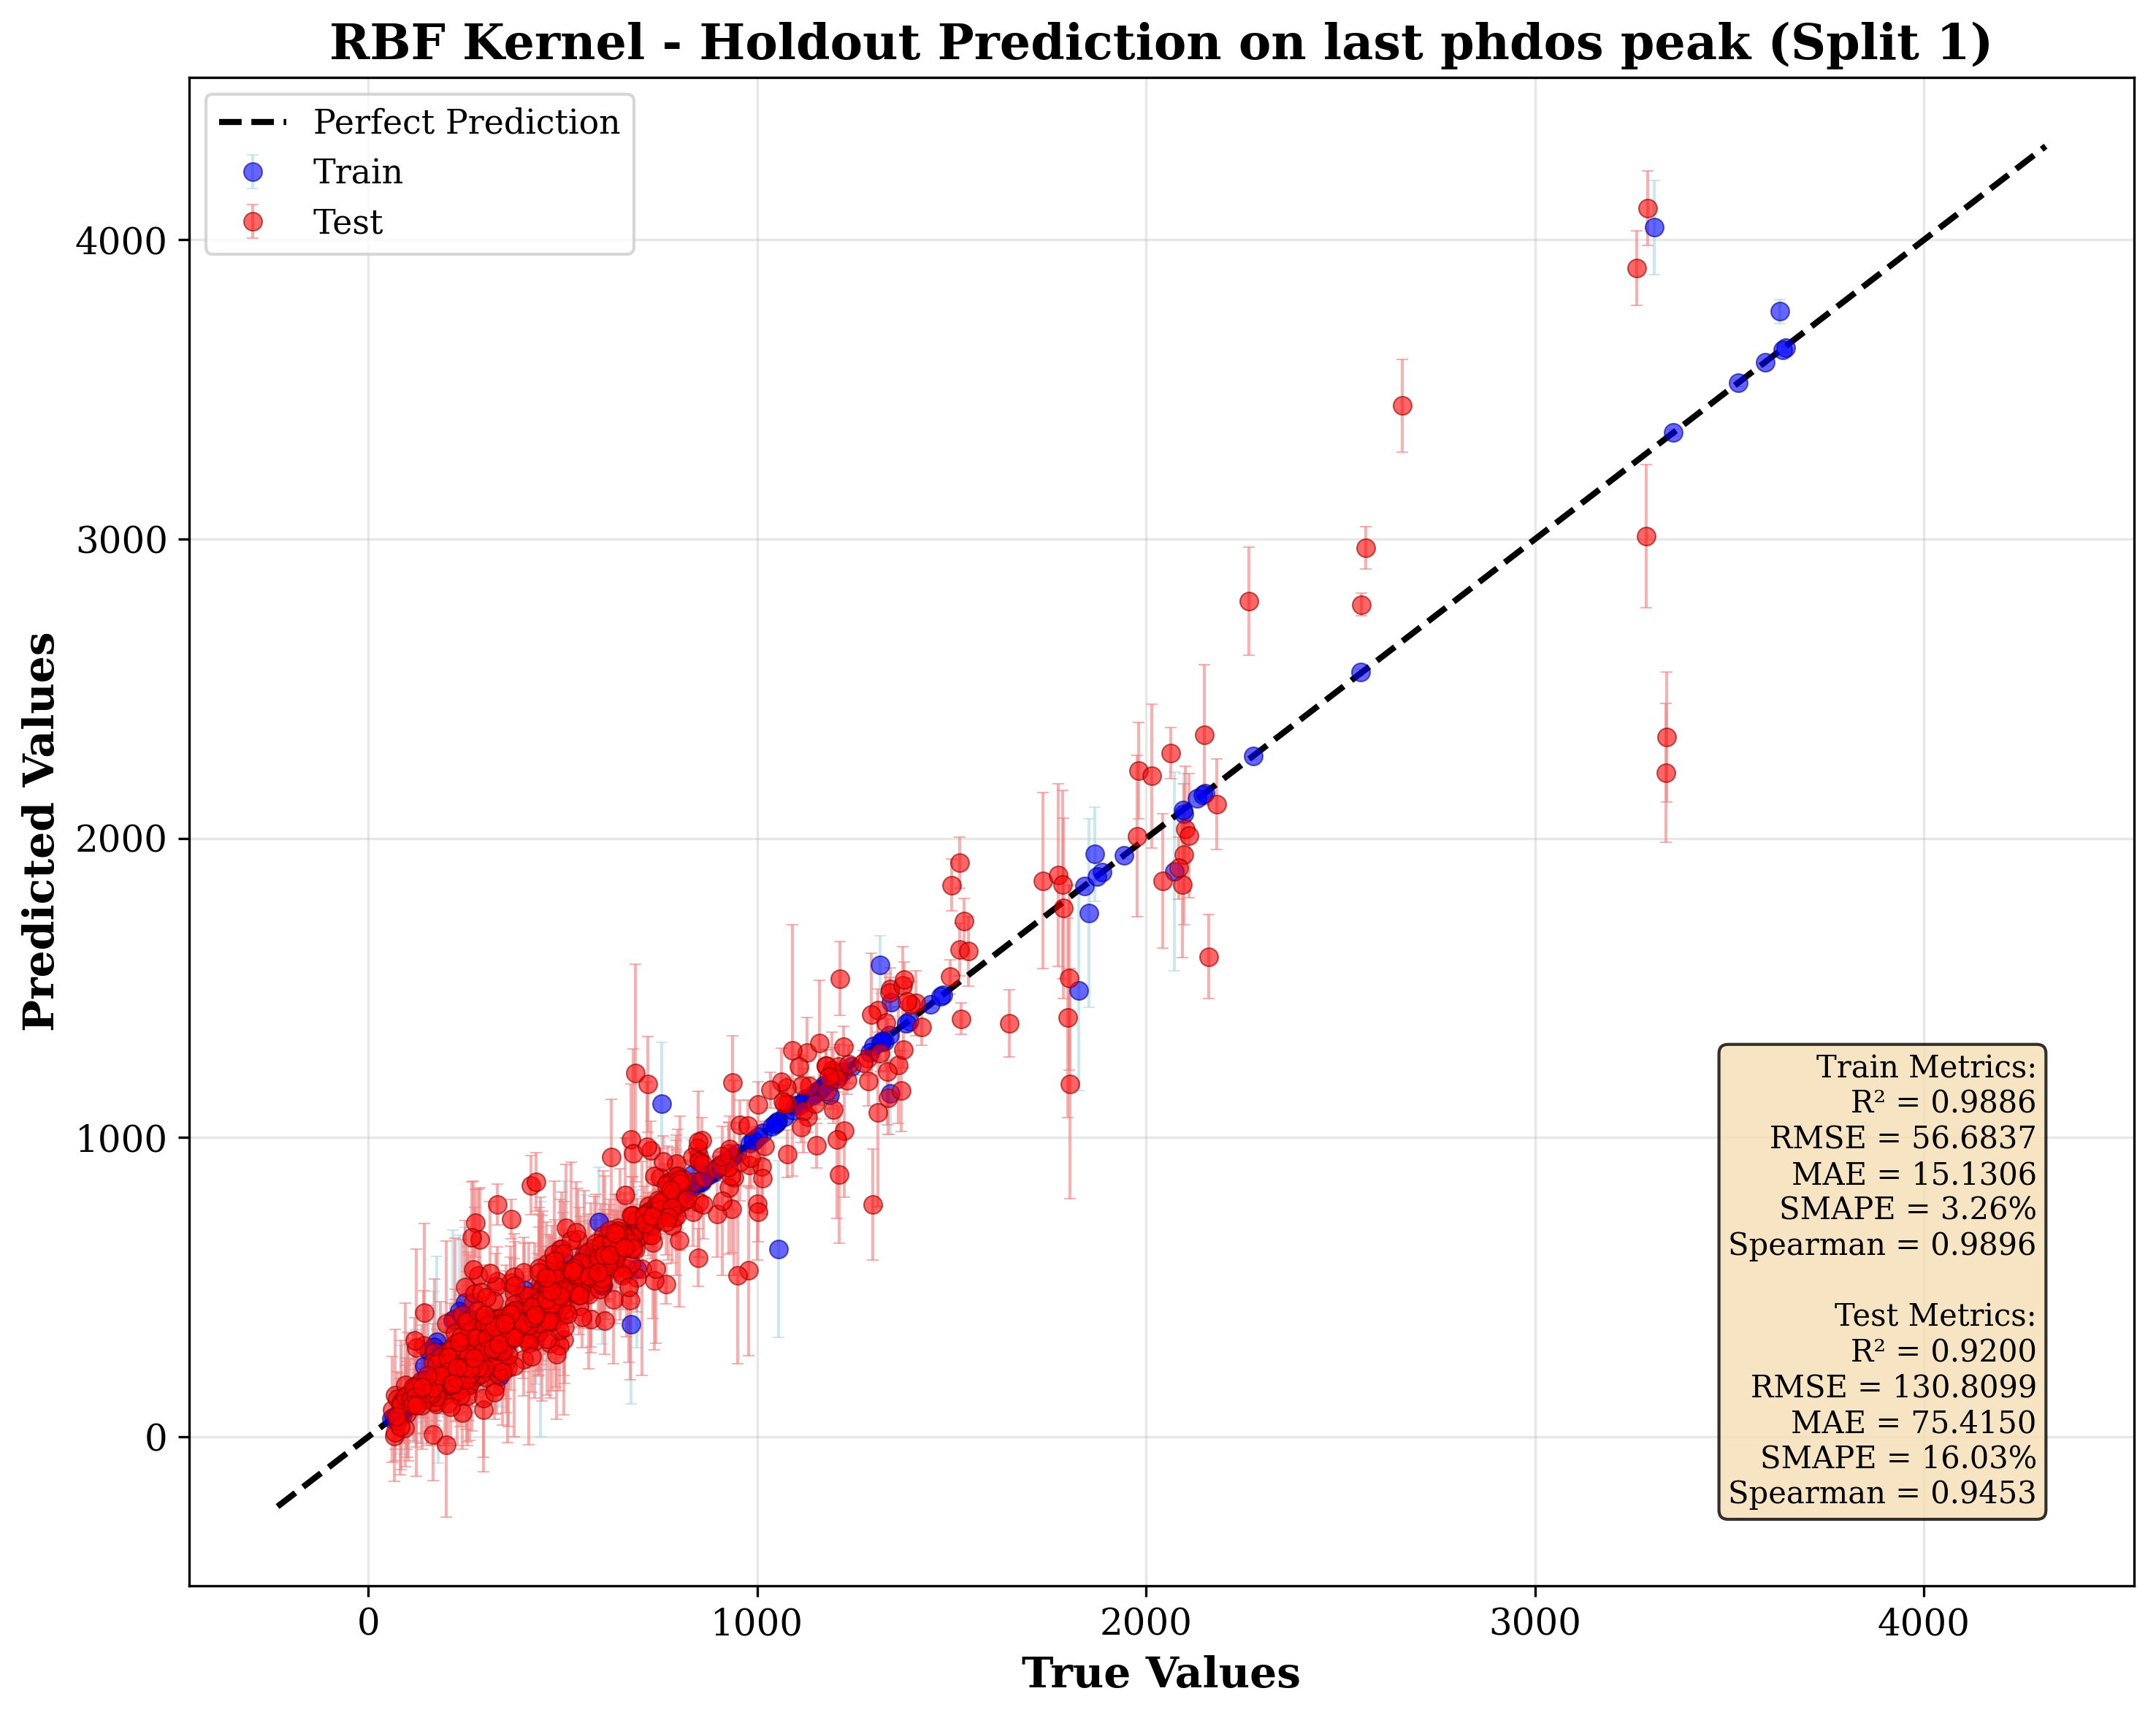
\includegraphics[width=\textwidth]{figures/fig_parity_phonon_phdos_peak_orb_gp.png}
        \caption{Phonon: phdos peak ($R^{2} = 0.911$)}
    \end{subfigure}
    \caption{Representative parity plots for the best-predicted property in each of the three benchmark datasets (ORB\,+\,GP, PCA\,=\,50, $\ntrain = 500$, split~1). All three show tight clustering around the diagonal with well-calibrated uncertainty bands.}
    \label{fig:parity_examples}
\end{figure*}

\FloatBarrier
\subsection{Cross-Dataset Synthesis}
\label{sec:cross_dataset}

Table~\ref{tab:cross_dataset} summarises the key findings across all three datasets, revealing both universal patterns and dataset-specific insights.

\begin{table*}[!htb]
    \centering
    \caption{Cross-dataset comparison at $\ntrain = 500$. For each dataset, we report the best configuration and its averaged metrics, together with the easiest and hardest properties.}
    \label{tab:cross_dataset}
    \footnotesize
    \begin{tabular}{@{}llccll@{}}
        \toprule
        \textbf{Dataset} & \textbf{Best Config} & \textbf{Avg.\ \Rtwo{}} & \textbf{Avg.\ $\rho$} & \textbf{Easiest Property} & \textbf{Hardest Property} \\
        \midrule
        Elastic tensor & ORB+DGP+PCA25 & 0.807 & 0.826 & $K_{\text{Voigt}}$ (0.931) & Poisson (0.658) \\
        Dielectric     & DGP+ORB+PCA10 & 0.336 & 0.778 & band\_gap (0.852) & poly\_elec ($-$0.180) \\
        Phonon dielec. & GP+ORB+PCA50  & 0.303 & 0.824 & phdos\_peak (0.911) & eps\_elec ($-$0.001) \\
        \bottomrule
    \end{tabular}
\end{table*}

Figure~\ref{fig:cross_descriptor} visualises this comparison: for each descriptor, we show the best achievable \Rtwo{} and Spearman~$\rho$ across all three datasets, with the name of the best-performing surrogate overlaid on each bar.

\begin{figure*}[!htb]
    \centering
    \begin{subfigure}[t]{0.48\textwidth}
        \centering
        
\includegraphics[width=\textwidth]{figures/fig_cross_dataset_R2_by_descriptor.png}
        \caption{Best \Rtwo{} per descriptor (label = best surrogate)}
        \label{fig:cross_desc_r2}
    \end{subfigure}
    \hfill
    \begin{subfigure}[t]{0.48\textwidth}
        \centering
        
\includegraphics[width=\textwidth]{figures/fig_cross_dataset_spearman_by_descriptor.png}
        \caption{Best Spearman~$\rho$ per descriptor (label = best surrogate)}
        \label{fig:cross_desc_spearman}
    \end{subfigure}
    \caption{Cross-dataset comparison of best achievable performance per descriptor at $\ntrain = 500$. Each bar shows the best \Rtwo{} (a) or Spearman~$\rho$ (b) across all surrogate--PCA combinations, with the winning surrogate name overlaid. ORB achieves the highest \Rtwo{} on all three datasets. Spearman correlations are consistently $>$0.7 for ORB across all datasets, confirming its utility for BO even when \Rtwo{} is low.}
    \label{fig:cross_descriptor}
\end{figure*}

Three universal patterns emerge:

\textbf{Pattern 1: ORB dominance.}
ORB is the best featuriser on every dataset, every surrogate, and nearly every individual property.
Its advantage is largest on the elastic dataset ($\Delta R^2 \approx 0.07$ over UMA/MACE) and smallest on the phonon dataset ($\Delta R^2 \approx 0.03$), but it never loses.
This consistency strongly supports ORB as the default featuriser for materials BO.

\textbf{Pattern 2: DGP fragility.}
The DGP collapses at PCA\,=\,50 on all three datasets, regardless of featuriser.
This is not a coincidence: the variational inference in the two-layer DGP involves $O(d^2)$ parameters in the hidden layer, and at PCA\,=\,50 with $\ntrain = 500$, the model is severely over-parameterised.
At PCA\,$\leq$\,25, the DGP can match or exceed the GP, but the risk of catastrophic failure makes it unreliable.

\textbf{Pattern 3: Spearman outperforms \Rtwo{}.}
Across all datasets, Spearman rank correlations are substantially higher than \Rtwo{} values.
This is most dramatic on the phonon dataset, where $\bar{R}^2 = 0.303$ but $\bar{\rho} = 0.824$.
For Bayesian optimisation, where the acquisition function depends on relative rankings, this means that even ``poorly'' fitting surrogates (by \Rtwo{}) can effectively guide the search.

Beyond these universals, we find dataset-specific insights.
On the elastic dataset, the property hierarchy (bulk modulus $>$ shear modulus $>$ anisotropy $>$ Poisson's ratio) mirrors the physical hierarchy of sensitivity to geometric vs.\ electronic structure.
On the dielectric dataset, band gap and refractive index are reasonably predicted because they correlate with bonding character, while the polycrystalline dielectric constants require many-body electronic structure information beyond geometric embeddings.
On the phonon dataset, the extreme \Rtwo{}-Spearman gap for eps\_electronic ($R^2 = -0.001$, $\rho = 0.930$) suggests that log-transforming or robust-scaling the target before training could dramatically improve \Rtwo{} without sacrificing ranking ability.

\FloatBarrier
\subsection{Closed-Loop Probe with Diffusion Backbones}
\label{sec:closed_loop_probe}

The static benchmark predicts an ORB\,+\,GP surrogate should remain useful in closed-loop Bayesian optimisation (BO) when $R^{2}$ is low but $\rho$ is high.
We tested this with three architecturally distinct pretrained diffusion priors, fine-tuned online via the policy-gradient procedure of MatInvent~\cite{chen2025matinvent}, with a Gaussian Process surrogate inserted between the SUN-filter and the property oracle.
The reinforcement-learning side of the procedure follows the lineage of DDPO~\cite{black2023ddpo} and DPOK~\cite{fan2023dpok} from the image domain, ported to crystals by MatInvent and (concurrently, for an autoregressive transformer prior) by CrystalFormer-RL~\cite{cao2025crystalformerrl}.
Existing tutorials and reviews of RL fine-tuning of diffusion models~\cite{uehara2024rldiffusion} catalogue several policy-gradient and value-based families, none of which include a Bayesian-optimisation gate at acquisition time; the recent npj Comp Mat review of generative AI for crystals~\cite{generative_review_2025} surveys the design space without devoting a section to closed-loop, online surrogate-gated refinement, although it does note one offline precedent---Qi et al.'s Latent Conservative Objective Models (LCOM)~\cite{qi2023lcom}, which trains a conservative surrogate over a CDVAE latent space to minimise formation energy.
LCOM differs from the present work in being offline (no online policy update of the generator), single-property (formation energy), and built around a CDVAE rather than a diffusion prior; we view it as a complementary precedent rather than a baseline.
The probe in this section sits in that gap.

We ran two property targets ($C_p$ and $K_{\text{VRH}}$), two policies (BASE and ACC, defined below), three backbones, and five seeds---thirty closed-loop runs in total, with a matching set for the bulk-modulus target.
The diffusion priors are not retrained from scratch; they are updated only through online REINFORCE-style rollouts.
The oracle is itself a learned surrogate (eSEN-30M-OAM~\cite{uma2025} fed into phonopy~\cite{togo2015first} for $C_p$ and a Birch--Murnaghan fit~\cite{birch1947finite} for $K_{\text{VRH}}$), and top candidates are not DFT-validated here.
With those caveats noted, the runs are large enough to examine cross-backbone behaviour, characterise the GP surrogate as the loop progresses, and report the practical effect of inserting the gate into a published RL pipeline.

\subsubsection{Pipeline and Setup}
\label{sec:cl_pipeline}

The three backbones are MatterGen~\cite{zeni2025mattergen} (\texttt{mg}), CrystalFlow~\cite{luo2025crystalflow} (\texttt{cf}), and ADiT~\cite{joshi2025adit} (\texttt{adit}).
Each runs under two policies.
BASE follows the published MatInvent recipe~\cite{chen2025matinvent} verbatim: policy-gradient updates with reward-weighted KL regularisation against the pretrained prior ($\sigma = 0.025$), an experience-replay buffer (size 100, sample size 10, reward cutoff 0.1), and a diversity filter on the long-term memory (tolerance 3, buffer 6).
ACC differs from BASE only in the property calculator: between the SUN filter and the oracle it inserts a Gaussian Process surrogate over ORB\,+\,PCA50 features, scores SUN-survivors by the acquisition rule (Expected Improvement plus a Determinantal Point Process diversity term), and dispatches only the top $K = 4$ to the oracle each cycle; the remaining candidates receive NaN reward, so they do not contribute to the policy-gradient update.
Every other RL hyperparameter (KL coefficient, replay buffer, diversity filter, finetune epochs, batch size $\sim 16$ candidates per cycle) is byte-identical between BASE and ACC.
Each run lasts 20 cycles, and every candidate passes the Stable+Unique+Novel (SUN) screen before any oracle or surrogate call.

\begin{figure}[H]
    \centering
    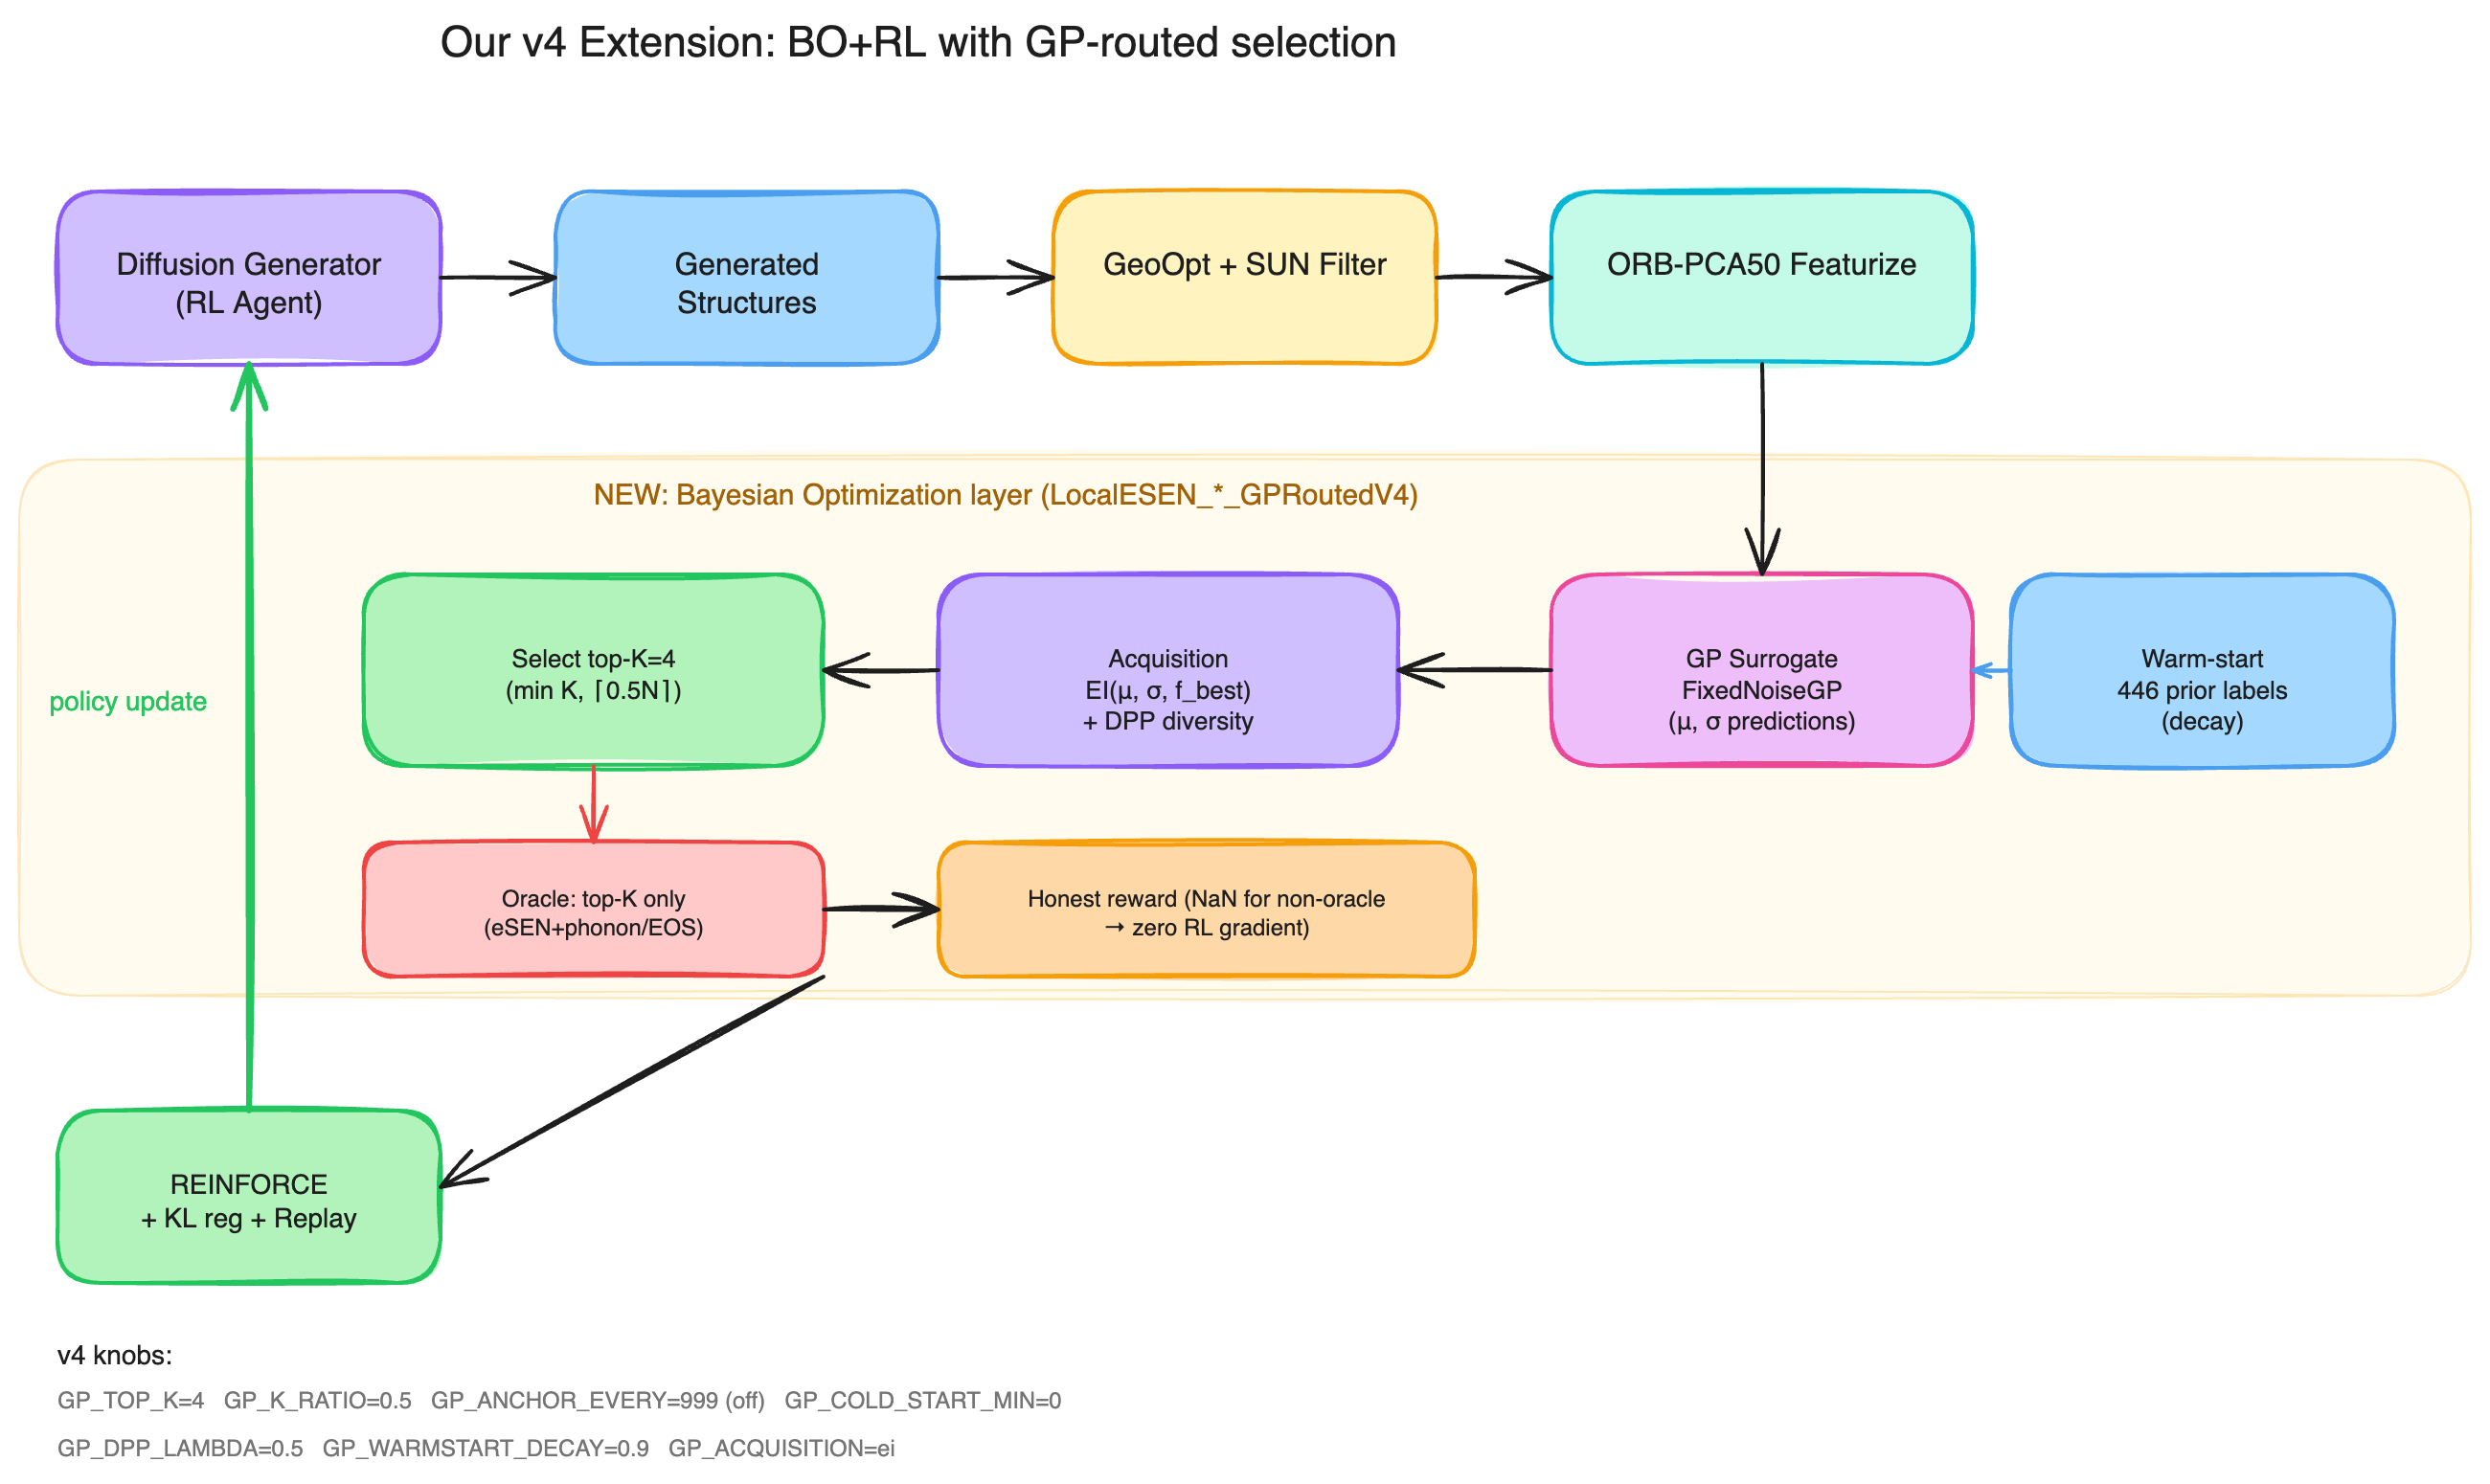
\includegraphics[width=\columnwidth]{figures/fig_closed_loop_pipeline.png}
    \caption{The closed-loop pipeline. The diffusion generator proposes structures; geometry optimisation and a SUN filter remove unstable, duplicate, or non-novel candidates; ORB\,+\,PCA50 featurises the survivors; the GP scores them; an acquisition rule (EI plus a DPP diversity term) selects the top $K=4$; only those reach the oracle (eSEN+phonon for $C_p$, EOS fit for $K_{\text{VRH}}$); REINFORCE then updates the diffusion policy. Non-oracle candidates receive NaN rewards and contribute zero RL gradient, so the surrogate's choice of which $K$ to call is the only training signal.}
    \label{fig:closed_loop_pipeline}
\end{figure}

\FloatBarrier
\subsubsection{Discovery Curves Across Backbones}
\label{sec:cl_curves}

Figure~\ref{fig:closed_loop_curves} tracks the running best property value over the 20 cycles, broken out by backbone and policy; per-seed running-bests are forward-filled to the full cycle horizon before averaging so that the cross-seed mean is itself non-decreasing.
For $C_p$, ACC reaches 1.0--1.2~J/g/K---approaching but short of the 1.5~J/g/K reference---in all three backbones, and exceeds BASE consistently in MatterGen, ADiT, and (more modestly) CrystalFlow.
For $K_{\text{VRH}}$, MatterGen and ADiT plateau near 310~GPa under ACC; the single best structure (375~GPa) is an MoN polymorph in space group $P\,\bar{6}m2$ (\#187) found by ADiT/ACC at seed 7.
CrystalFlow shows the largest between-seed spread of the three backbones for both targets, so its mean comparison is the noisiest of the panel, but the ACC mean still sits above the BASE mean throughout.
The qualitative pattern is consistent with the static-benchmark prediction in Section~\ref{sec:spearman_r2}: a high-$\rho$, low-\Rtwo{} surrogate suffices to drive acquisition without breaking the underlying RL update.
Trajectories at cycle 20 are also consistent with the published MatInvent runs at the equivalent loop count---Fig.~2c of \cite{chen2025matinvent} (10-seed mean) shows a heat-capacity mean of roughly 0.7--0.9~J/g/K at loop 20 in their MatterGen-based setup, within the seed-level error bands of our 5-seed BASE run.

\begin{figure*}[!htb]
    \centering
    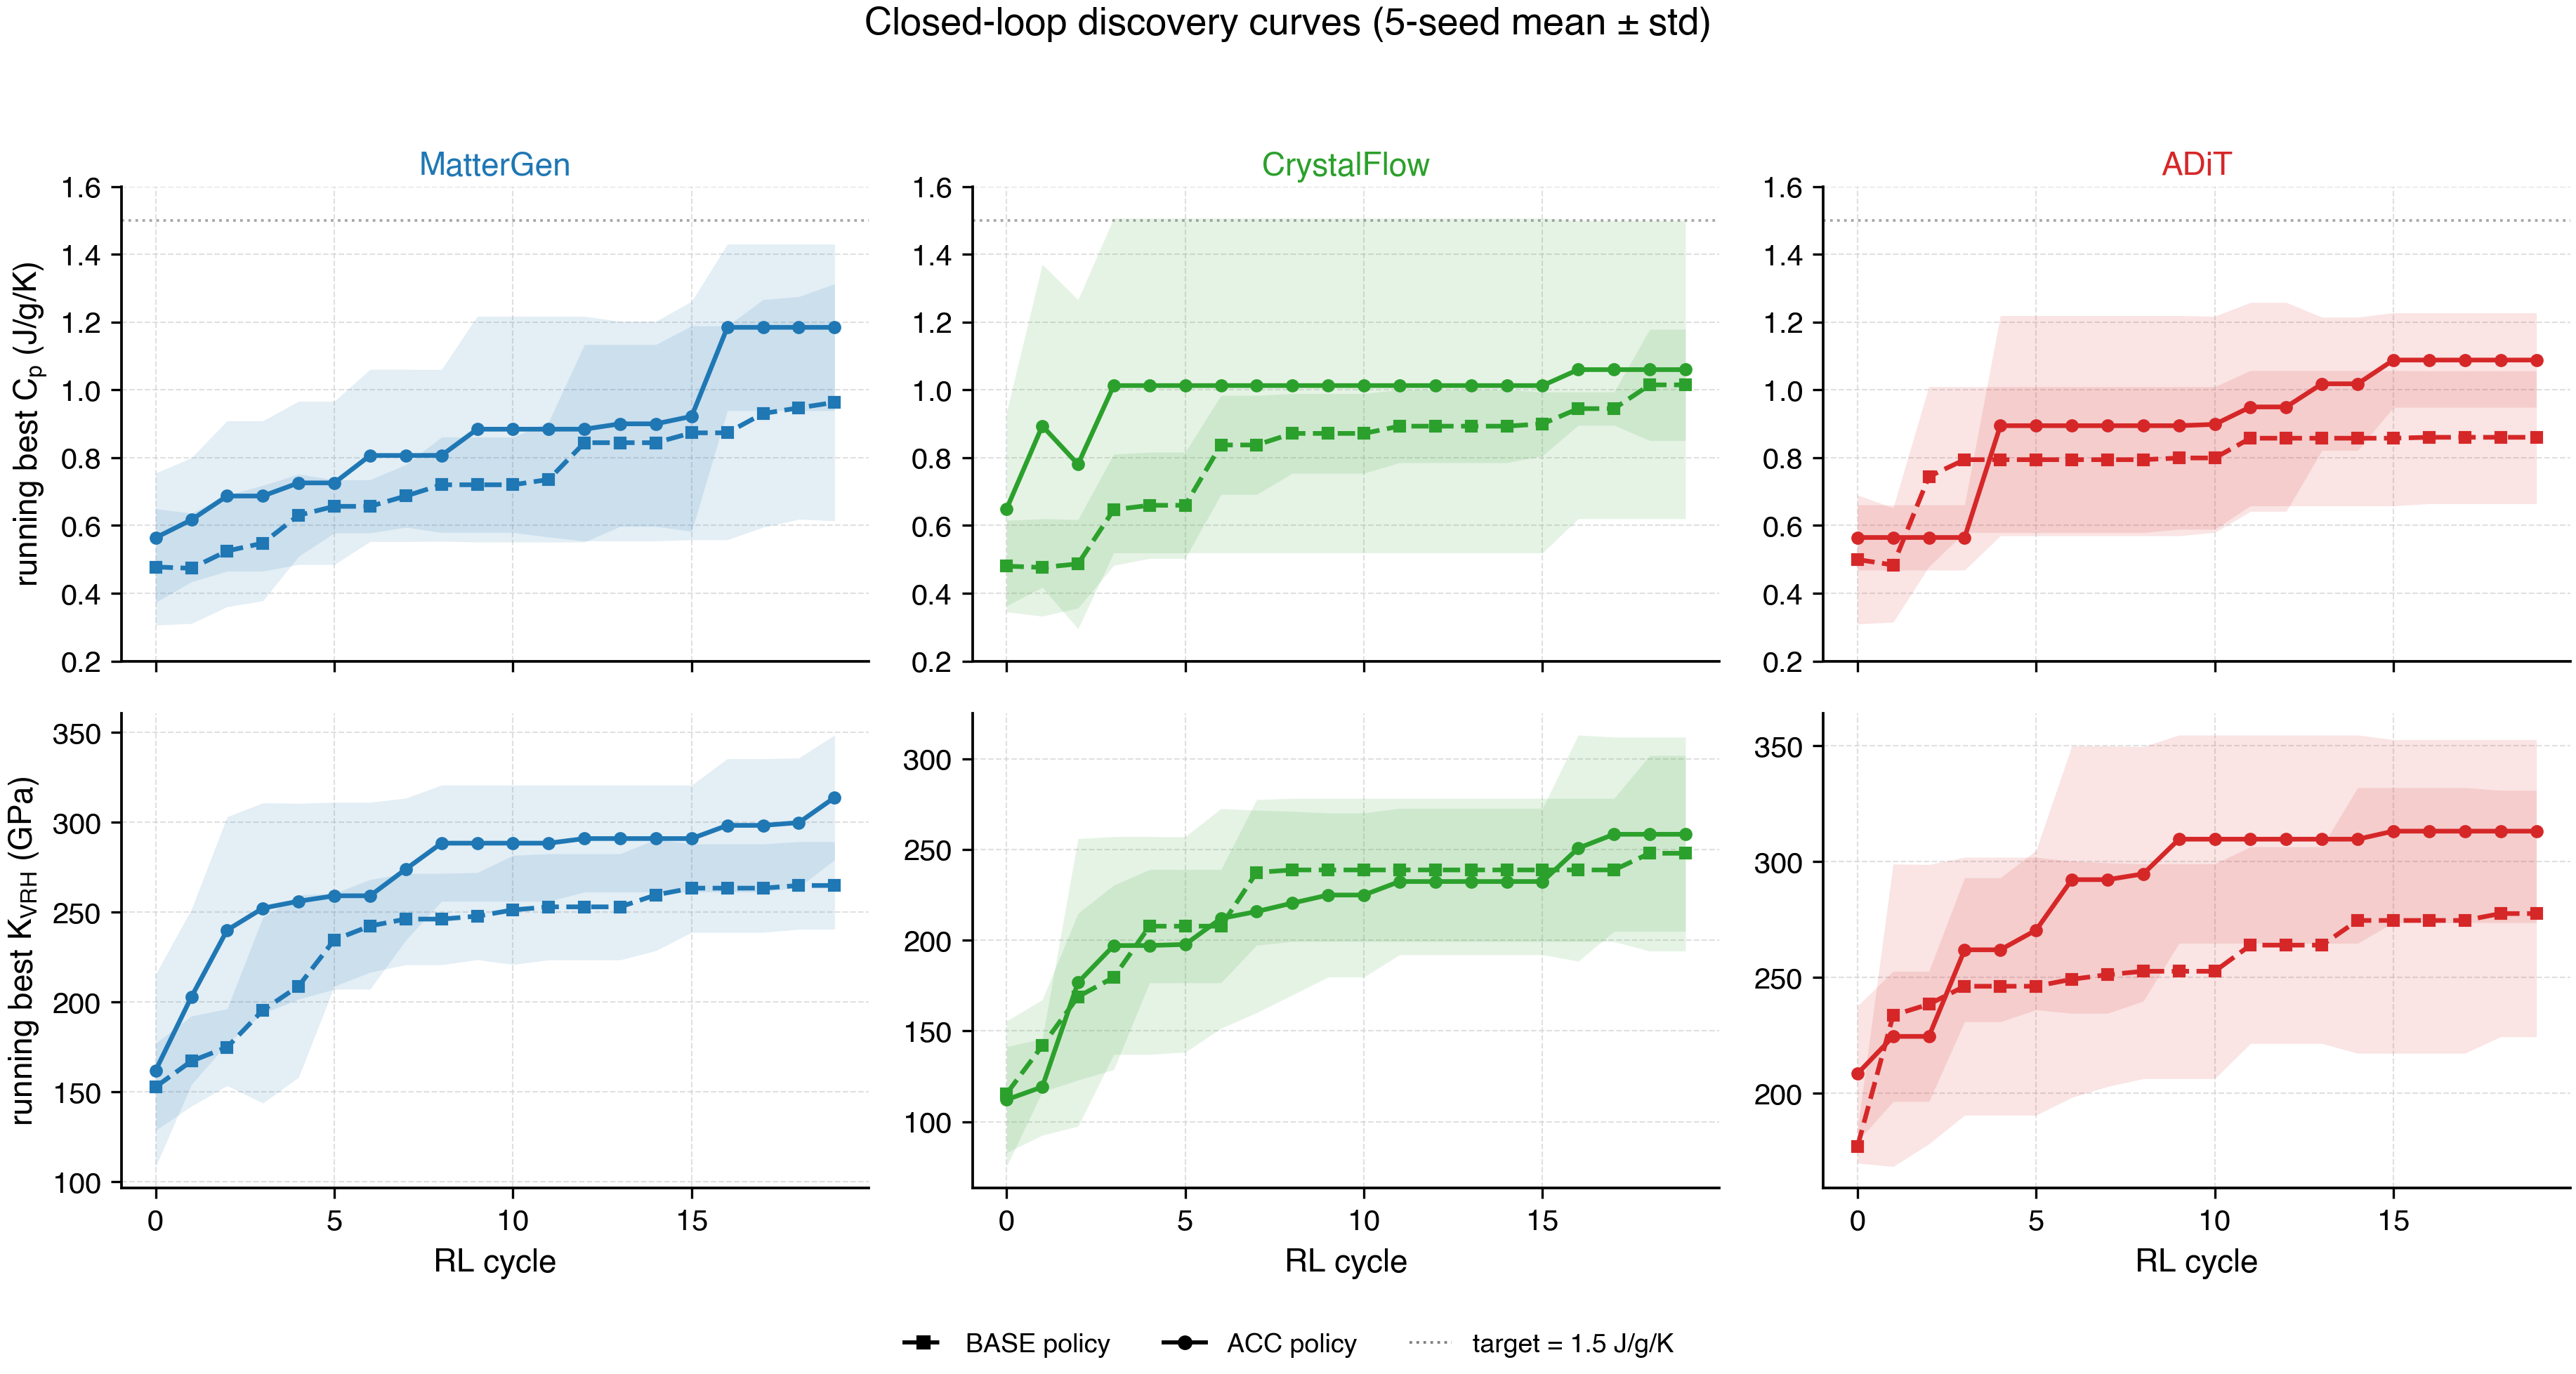
\includegraphics[width=\textwidth]{figures/fig_bogen_curves.png}
    \caption{Running best property value over 20 RL cycles, 5-seed mean $\pm$ std. Top row: $C_p$ (target $\to$ 1.5~J/g/K, dotted line). Bottom row: $K_{\text{VRH}}$ (max). Solid lines and circles: GP-gated BO (ACC); dashed lines and squares: vanilla REINFORCE (BASE). MatterGen and ADiT show a clean ACC-over-BASE lift on both targets; CrystalFlow's seed variance is too large to call either policy a winner.}
    \label{fig:closed_loop_curves}
\end{figure*}

\FloatBarrier
\subsubsection{Surrogate Quality Across Cycles}
\label{sec:cl_surrogate}

Figure~\ref{fig:closed_loop_surrogate} plots the GP CV5 RMSE per cycle, ACC runs only.
This metric is 5-fold cross-validation on the GP's accumulated training set---the oracled candidates from the warm-start plus all top-$K$ acquisitions up to the current cycle (16 points at cycle~0, growing by 4 per cycle to 92 by cycle 19).
It measures how well the GP fits its own oracled labels under leave-one-fold-out resampling; it does \emph{not} measure error on the next batch of fresh diffusion proposals, which is the quantity the gate actually uses $\mu$ to score.
On $C_p$ the CV5 RMSE sits at 0.075--0.090 (normalised property scale) and is statistically flat across cycles---mean RMSE in cycles 0--5 differs from cycles 15--19 by less than one between-seed standard deviation.
$K_{\text{VRH}}$ shows the same pattern at the 21--26~GPa level, with a mild downward trend in MatterGen and CrystalFlow.
The fair reading is that the GP remains internally consistent as the training set grows---the loop does not break self-consistency---which is a necessary but not sufficient condition for surrogate-gated BO health.
A held-out RMSE on the diffusion proposals before they reach the gate is not in our current logs; this is the metric we would need to claim true generalisation, and we flag its absence as a limitation in Section~\ref{sec:cl_caveats}.

\begin{figure*}[!htb]
    \centering
    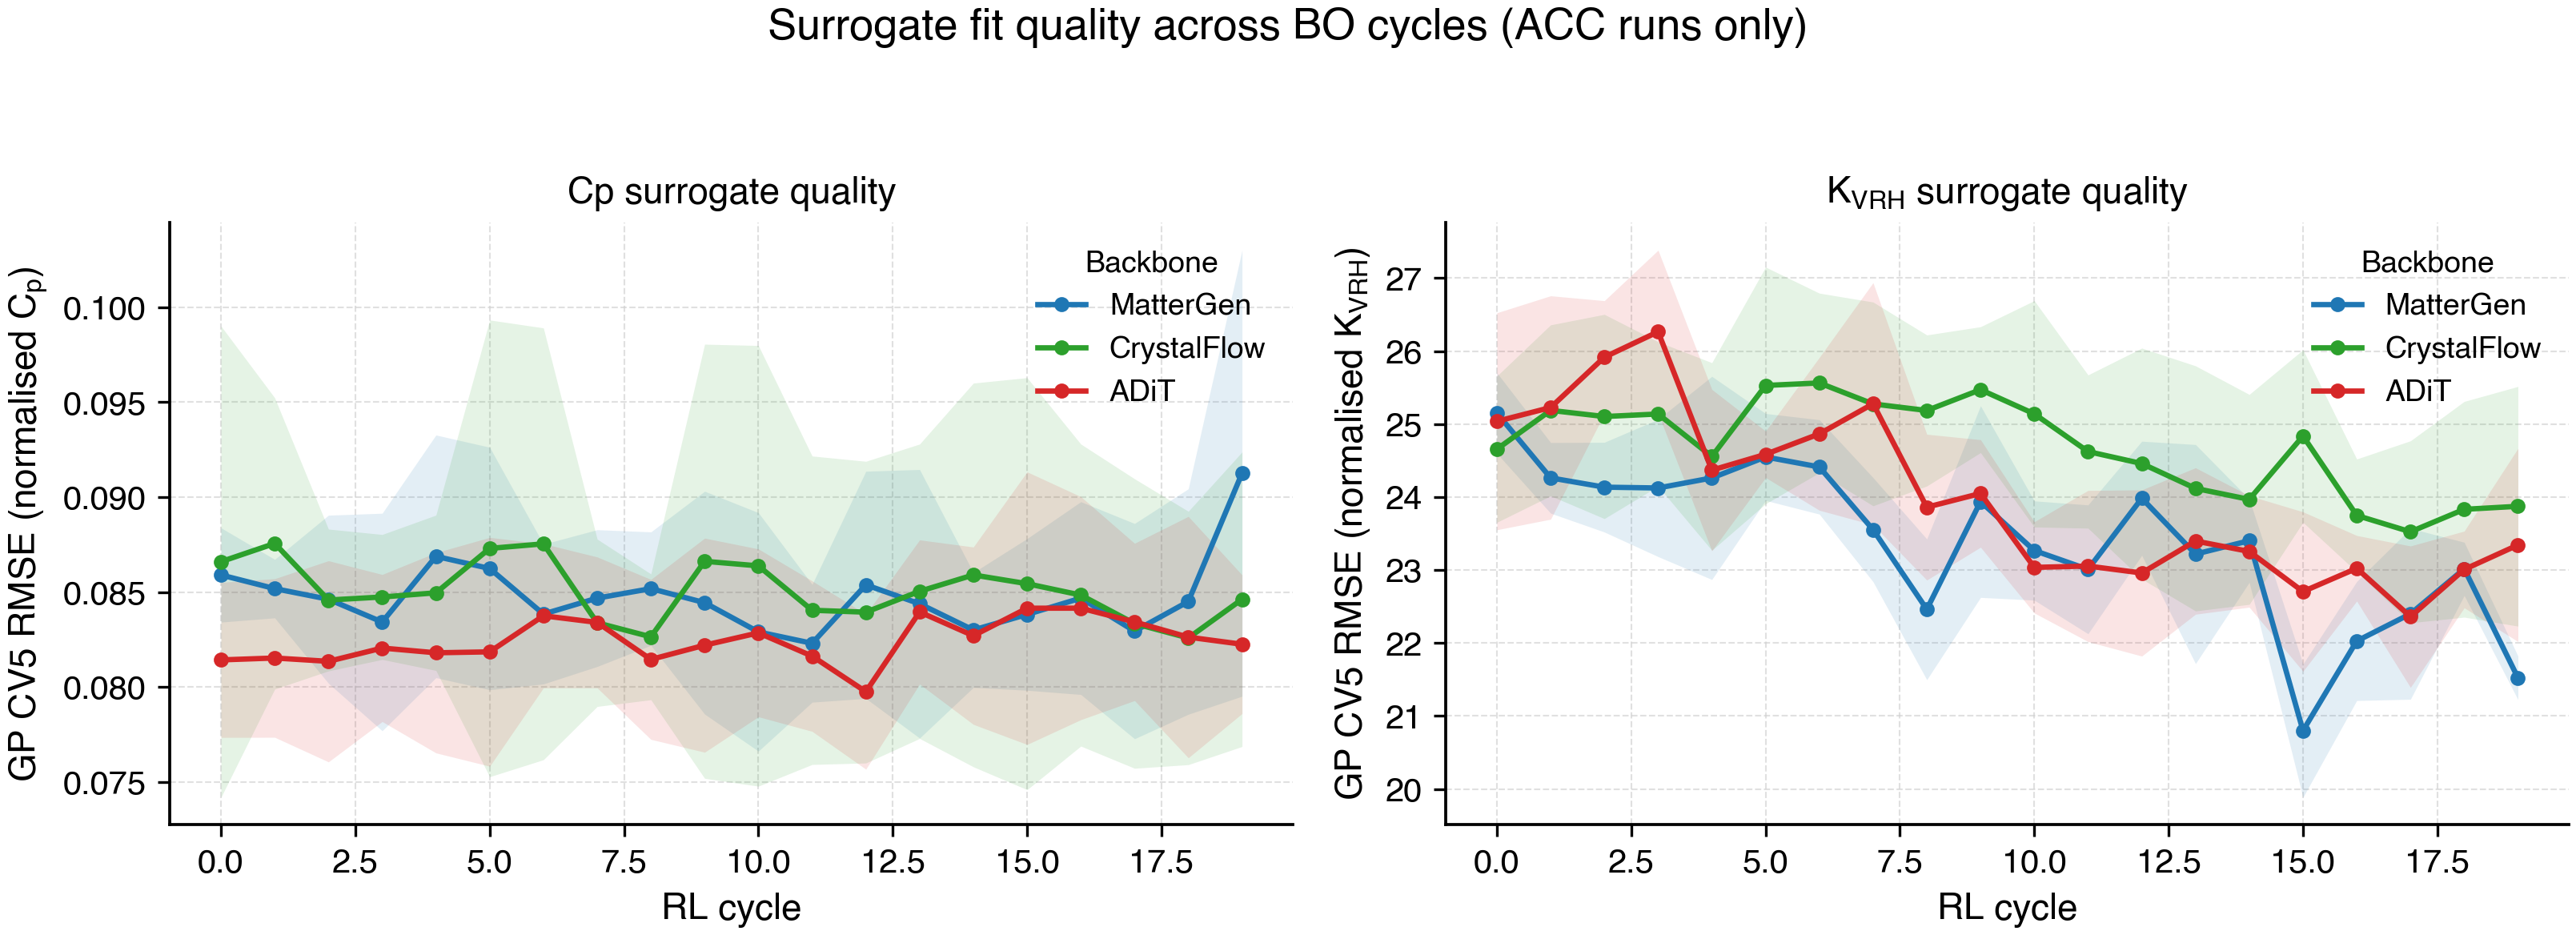
\includegraphics[width=\textwidth]{figures/fig_bogen_surrogate_quality.png}
    \caption{GP CV5 RMSE (normalised property scale) per RL cycle, ACC runs only, mean $\pm$ std across 5 seeds. CV5 is computed on the GP's accumulated oracled training set (16 points at cycle~0, growing to 92 by cycle 19), not on held-out fresh diffusion proposals. The flatness across cycles indicates that the loop does not break the GP's self-consistency as the training pool grows; it does not directly demonstrate generalisation to unseen candidates.}
    \label{fig:closed_loop_surrogate}
\end{figure*}

\FloatBarrier
\subsubsection{Oracle-Call Savings from the GP Gate}
\label{sec:cl_oracle}

The GP gate's practical payoff is that it caps the number of expensive oracle calls per cycle at $K=4$ regardless of how many candidates pass the SUN filter, replacing the rest with cheap GP-$\mu$ pseudo-evaluations.
Figure~\ref{fig:closed_loop_oracle_savings} compares cumulative oracle calls per run between BASE (every SUN-survivor goes to the oracle) and ACC (top-$K=4$ only) for both targets.
ACC's curve is the same straight line for every backbone---16 oracle calls for the warm-start at cycle 0, then 4 per cycle, totalling 92 calls per 20-cycle run.
BASE's curve depends on each backbone's SUN-survival rate.

Total oracle calls per run, 5-seed mean: for $C_p$, BASE/ACC is 169/92 in MatterGen ($1.83\times$ saving), 49/70 in CrystalFlow ($0.69\times$, i.e.\ ACC actually costs more), and 70/84 in ADiT ($0.83\times$); for $K_{\text{VRH}}$, BASE/ACC is 320/92 in MatterGen ($3.47\times$), 124/68 in CrystalFlow ($1.83\times$), and 206/83 in ADiT ($2.49\times$).
The pattern is consistent: where SUN survival per cycle exceeds $K=4$ (MatterGen on both targets, all backbones on $K_{\text{VRH}}$), the gate pays off; where survival is below $K$ (CrystalFlow and ADiT on $C_p$, where the unfiltered REINFORCE produces few stable+unique+novel candidates), BASE is naturally throttled and ACC's fixed $K$ raises rather than lowers the call count.
The trade-off in those low-throughput cases is not a saving in oracle calls but a saving in candidate quality: the gate forces a top-$K$ selection by EI\,+\,DPP rather than letting whatever survives SUN drift through to the oracle.

\begin{figure*}[!htb]
    \centering
    
\includegraphics[width=\textwidth]{figures/fig_bogen_oracle_savings.png}
    \caption{Cumulative oracle calls per closed-loop run, 5-seed mean $\pm$ std. ACC's straight line at +4 per cycle (after a warm-start of 16) reflects the fixed top-$K=4$ gate. BASE varies with each backbone's SUN-survival rate. The gate saves oracle calls for backbones with high SUN survival (MatterGen on both targets, all backbones on $K_{\text{VRH}}$, $1.8$--$3.5\times$ reduction); for low-survival backbones on $C_p$, ACC's fixed $K$ slightly raises the call count, with the trade-off being that the candidates picked are EI\,+\,DPP-selected rather than arbitrary SUN survivors.}
    \label{fig:closed_loop_oracle_savings}
\end{figure*}

\FloatBarrier
\subsubsection{Crystal-System Distribution of Generated Top Structures}
\label{sec:cl_crystal_systems}

The space groups of the top-3 candidates per run reveal a strong asymmetry across backbones (Figure~\ref{fig:closed_loop_spacegroup}).
For $C_p$, CrystalFlow and ADiT both produce more than half of their top structures in triclinic and monoclinic systems---the lowest-symmetry crystal classes---while MatterGen splits more evenly, contributing the bulk of the orthorhombic and tetragonal hits.
This is consistent with each prior's training distribution: MatterGen is trained on Materials Project ground-state structures (symmetry-rich), whereas the latent and flow priors more often emerge from optimisation in low-symmetry space.
For $K_{\text{VRH}}$ (Supporting Information) the dominance of low-symmetry systems persists, but cubic and hexagonal structures are over-represented relative to $C_p$, reflecting the well-known correlation between high bulk modulus and densely packed cubic/hexagonal lattices.
Splitting by policy (right panel) shows that the GP gate (ACC) does not bias the loop towards any particular crystal system---both BASE and ACC produce the same broad triclinic/monoclinic dominance, so the GP is screening on the property rather than on geometric proxies.

\begin{figure*}[!htb]
    \centering
    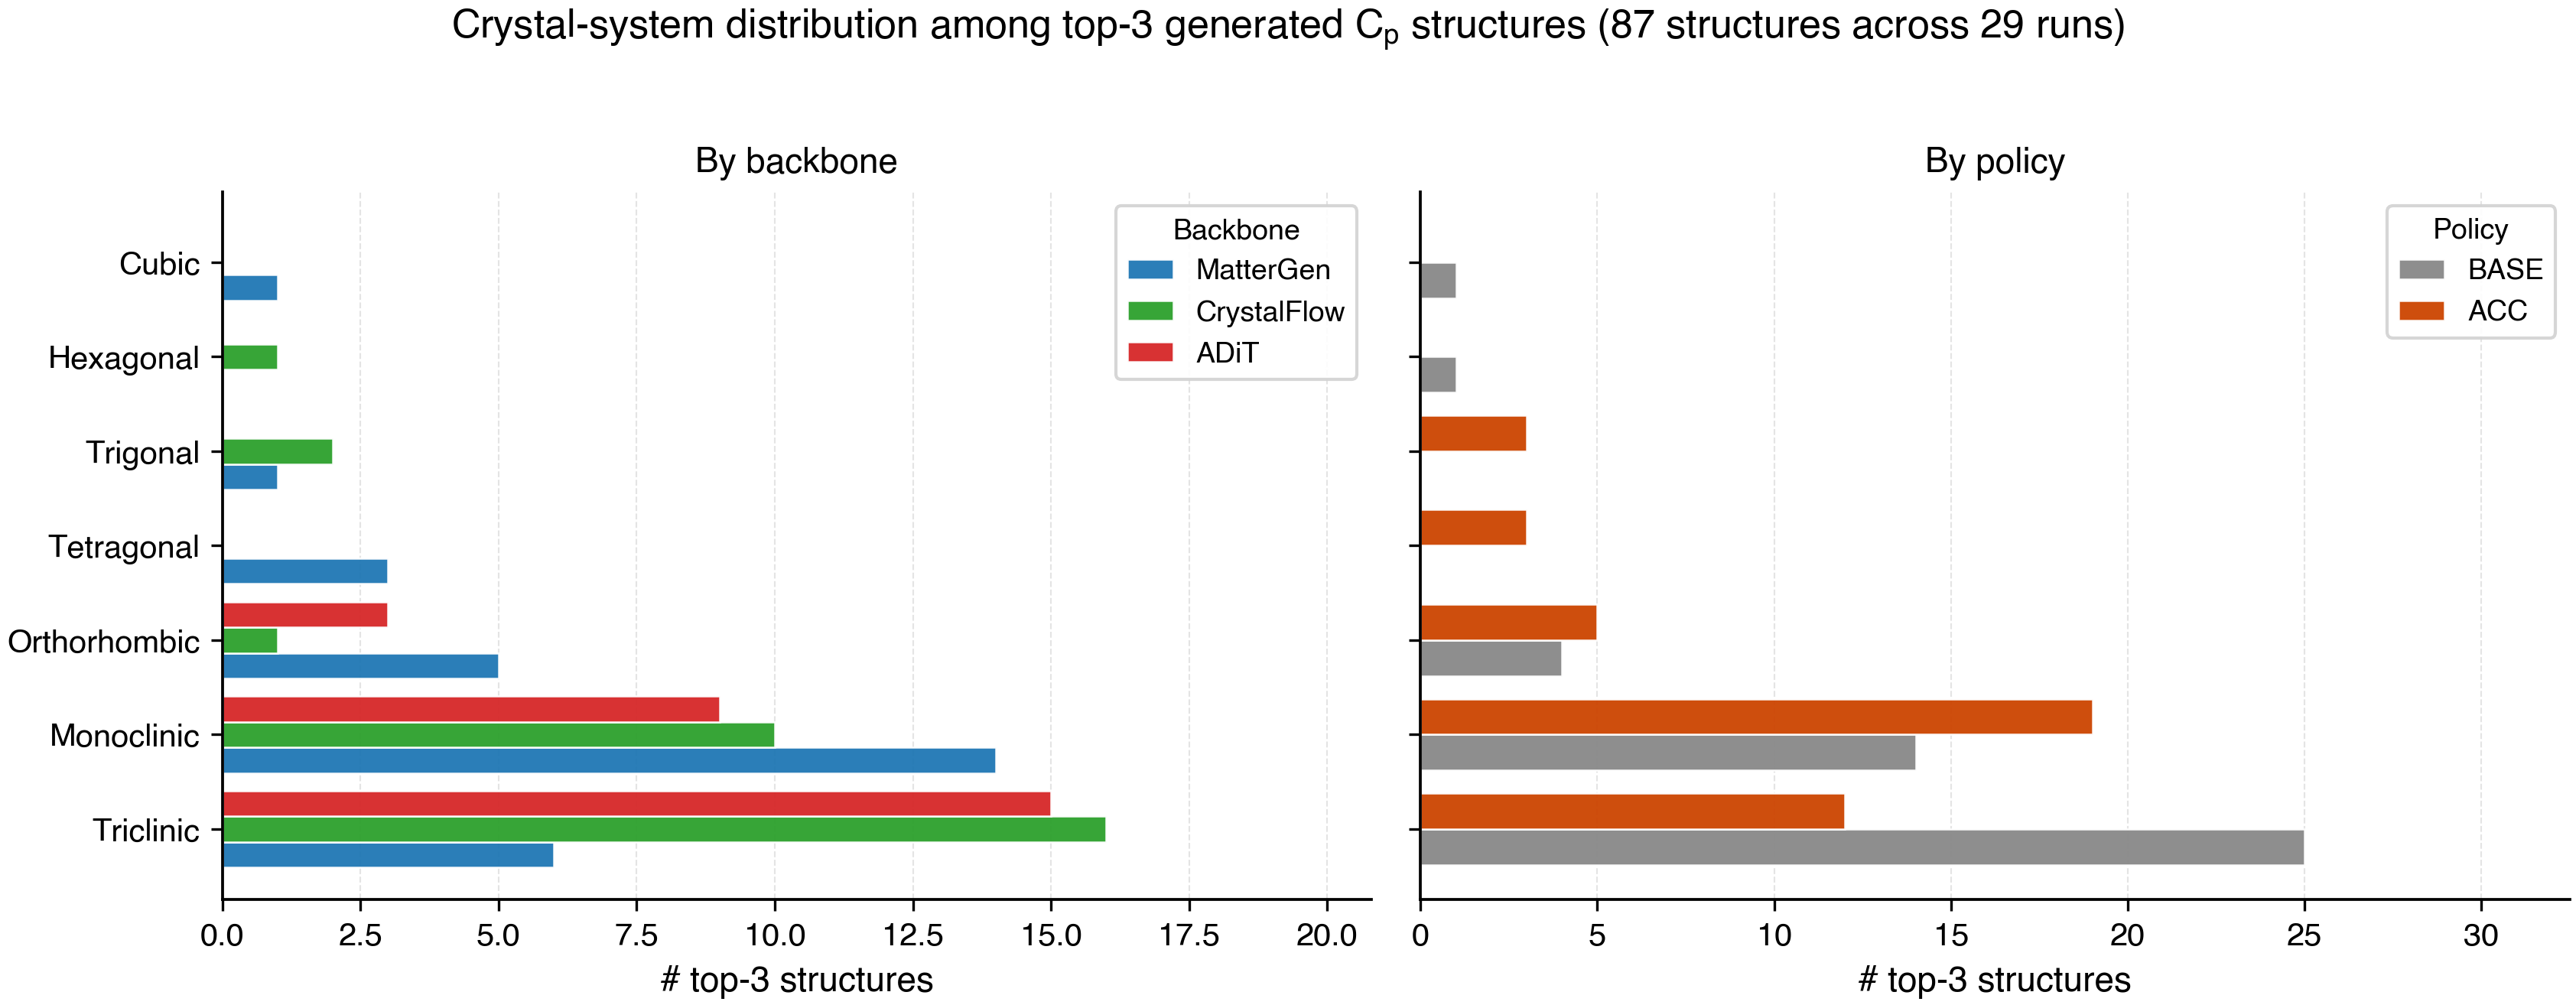
\includegraphics[width=\textwidth]{figures/fig_bogen_spacegroup_dist_cp.png}
    \caption{Crystal-system distribution among top-3 generated $C_p$ structures (87 structures across 30 runs). Left: by backbone. Right: by policy. CrystalFlow and ADiT skew strongly towards low-symmetry (triclinic, monoclinic) systems; MatterGen is the only backbone producing tetragonal hits; the BASE-vs-ACC split is balanced across systems, so the GP gate is property-driven, not geometry-driven. The matching $K_{\text{VRH}}$ panel is in the Supporting Information.}
    \label{fig:closed_loop_spacegroup}
\end{figure*}

\FloatBarrier
\subsubsection{Per-Backbone Summary}
\label{sec:cl_per_model}

Figure~\ref{fig:closed_loop_per_model} consolidates the headline numbers per backbone across all 30 runs.
Best-value bars (left column) split BASE vs.\ ACC: MatterGen and CrystalFlow both hit the 2.0~J/g/K reward ceiling (oracle-imposed cap, attained on a few seeds) while ADiT plateaus at 1.28~J/g/K; for $K_{\text{VRH}}$, ADiT's 375~GPa hit pulls its best-value bar above MatterGen's 340 and CrystalFlow's 336~GPa.
Mean top-3 (right column) is the more honest comparator because best-of-30 picks up lucky seeds: on $C_p$ the three backbones land at 1.11~$\pm$~0.56, 0.89~$\pm$~0.40, and 0.80~$\pm$~0.18~J/g/K---differences smaller than the within-backbone seed spread.
On $K_{\text{VRH}}$ the corresponding means are 273~$\pm$~37, 224~$\pm$~43, and 259~$\pm$~45~GPa, again with overlapping error bars.
Novelty against the warm-start seed pool is uniform across backbones at 100\% for $C_p$ and 96.7\% for $K_{\text{VRH}}$, so we report it verbally rather than as a separate panel; details and the formula-level analysis are in Section~\ref{sec:cl_novelty}.
The ACC-vs-BASE lift on best-of-30 is consistent in MatterGen and ADiT (Section~\ref{sec:cl_curves}) but never large enough to outweigh seed variance, so we report it as a trend rather than a measured difference.

\begin{figure*}[!htb]
    \centering
    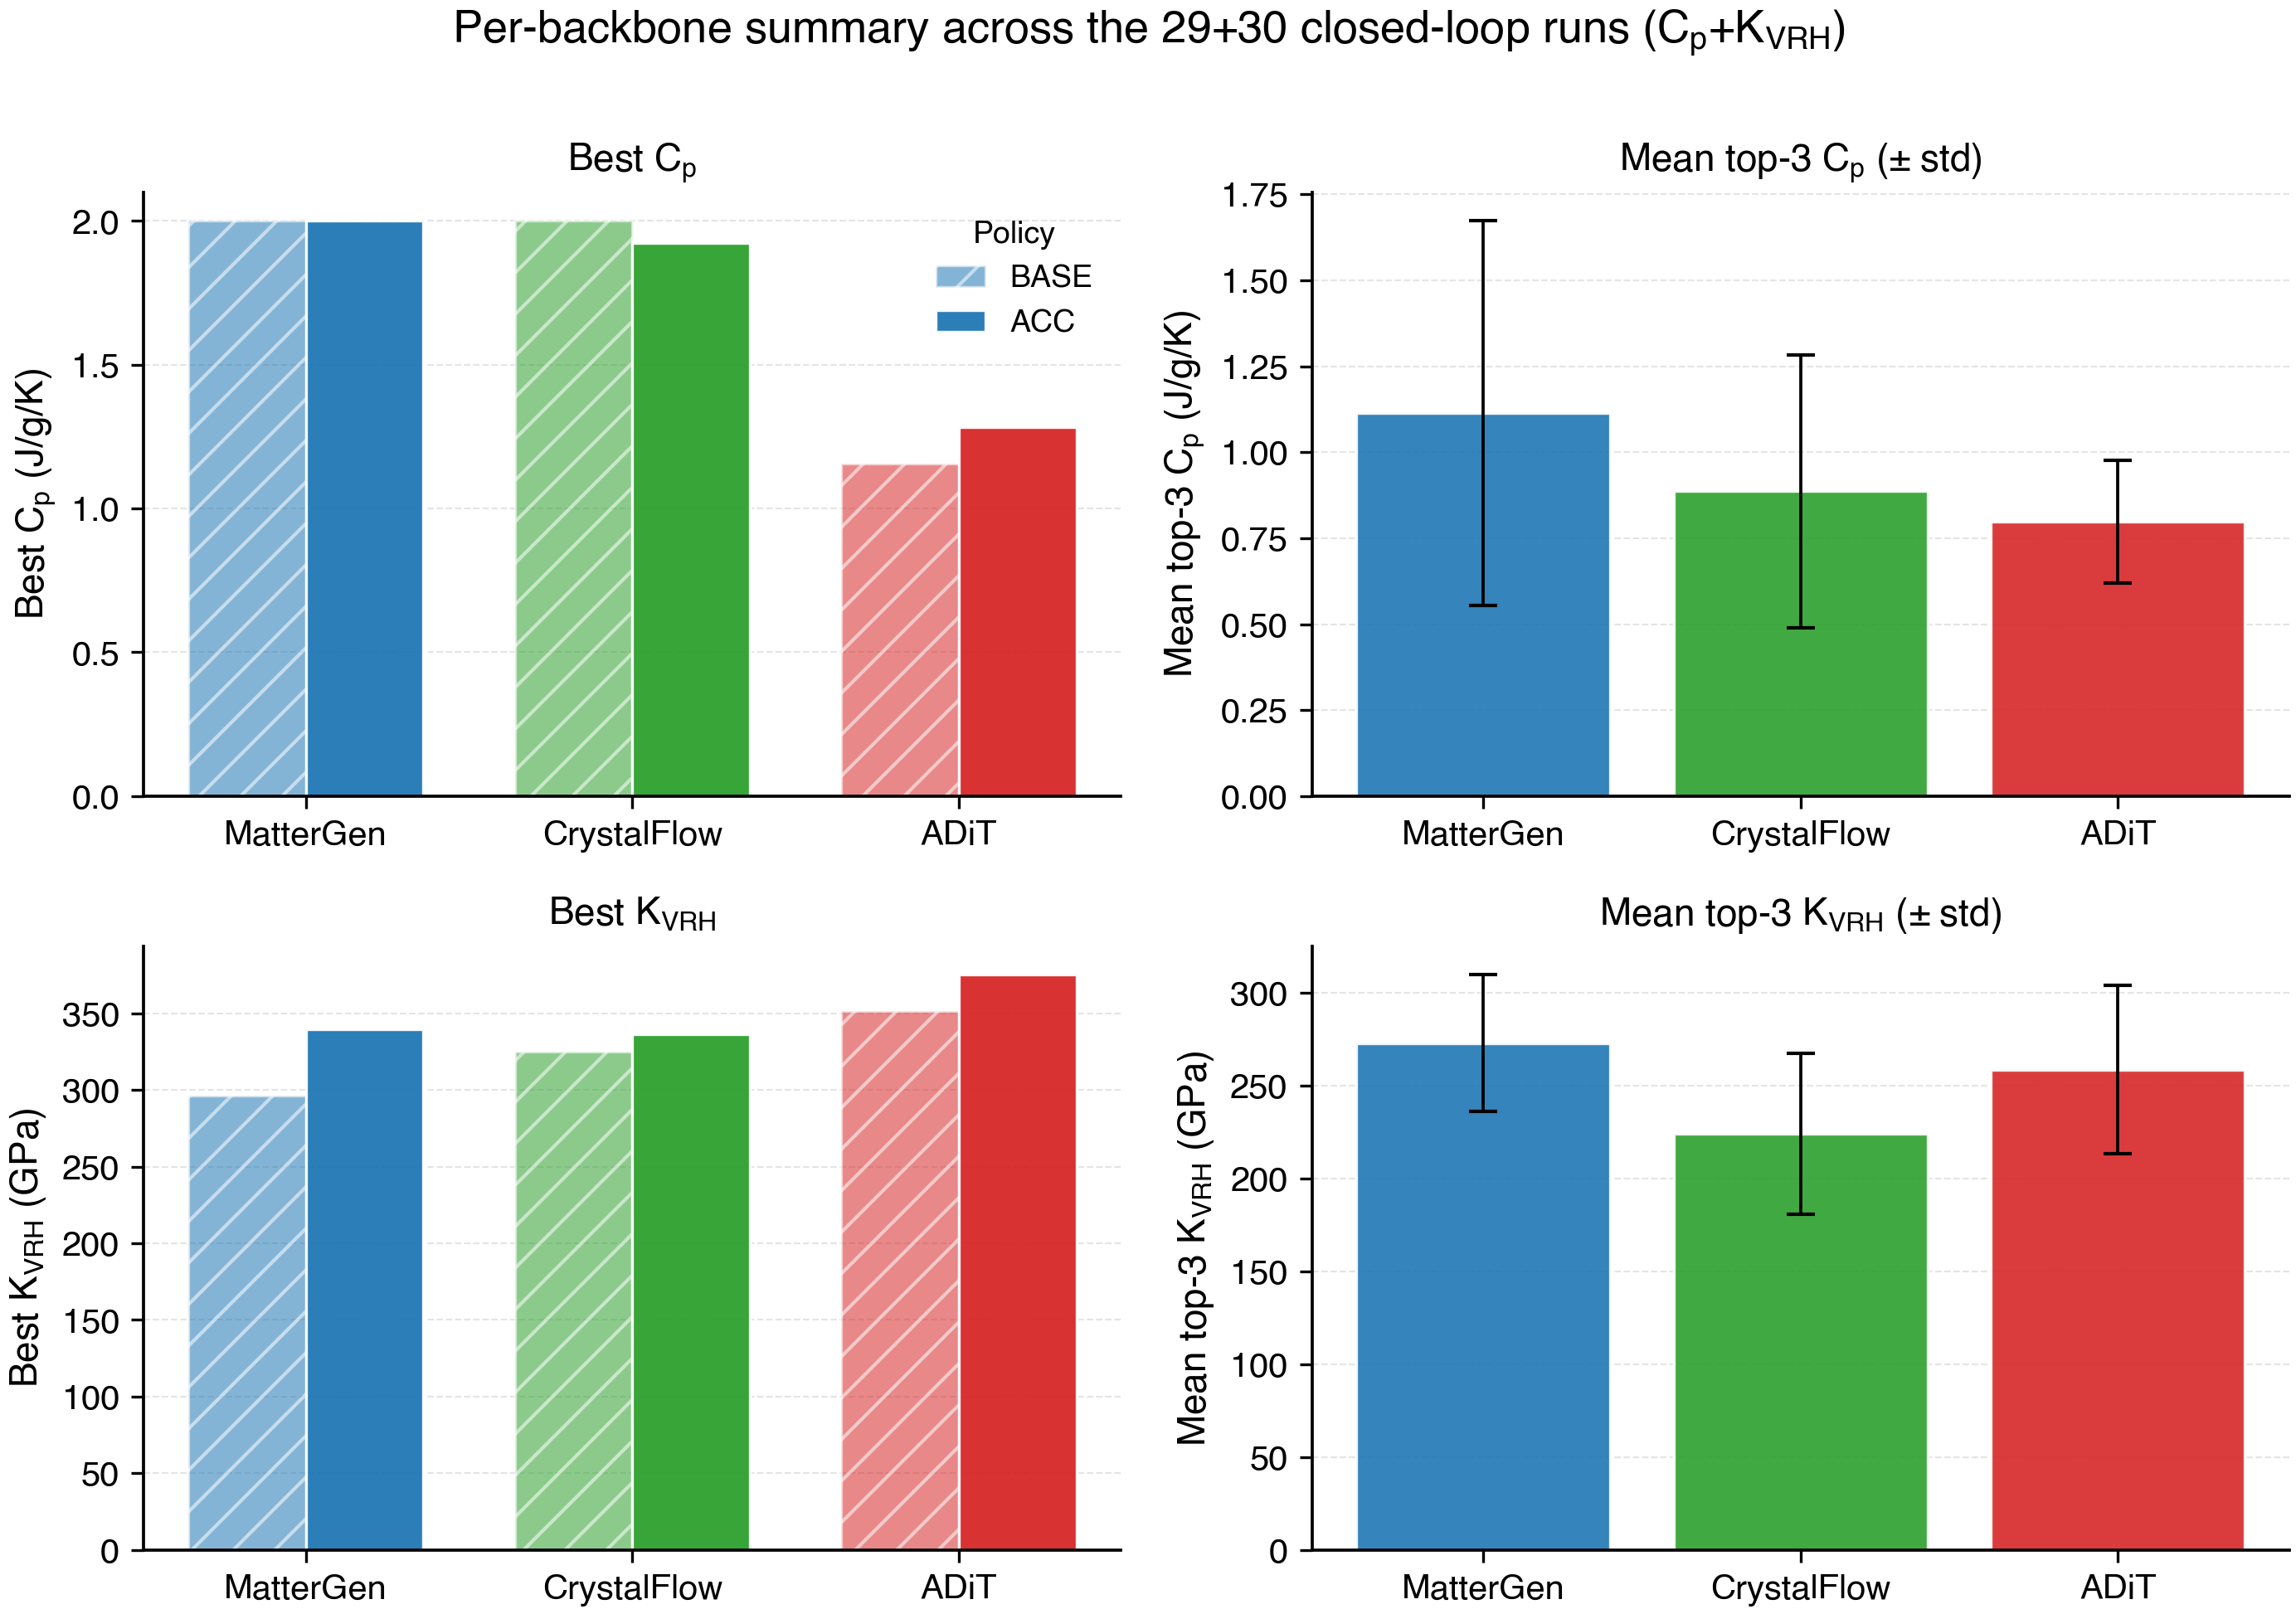
\includegraphics[width=0.85\textwidth]{figures/fig_bogen_per_model_summary.png}
    \caption{Per-backbone summary across the 30 closed-loop runs. Left column: best property value (hatched = BASE, solid = ACC). Right column: mean top-3 value $\pm$ std across runs. Top row: $C_p$. Bottom row: $K_{\text{VRH}}$. The best-value spread across backbones is small once seed variance is taken into account; ACC's lift over BASE is consistent but modest. Novelty rates against the warm-start seed pool are 100\% ($C_p$) and 96.7\% ($K_{\text{VRH}}$) for all three backbones (Section~\ref{sec:cl_novelty}).}
    \label{fig:closed_loop_per_model}
\end{figure*}

\FloatBarrier
\subsubsection{Novelty vs.\ the Warm-Start Seed Pool}
\label{sec:cl_novelty}

A natural worry is that the loop is retrieving the structures we used to warm-start the GP rather than producing new ones.
We checked this with \texttt{StructureMatcher}~\cite{pymatgen2013} at default tolerances.
For $C_p$, none of the 87 top-3 structures (aggregated across all 30 runs) shares a reduced formula with the seed pool, and zero pass strict matching.
For $K_{\text{VRH}}$, 3 of 90 share a reduced formula but again zero pass strict matching.
The GP is acting as a property prior, not as memory.

Figure~\ref{fig:closed_loop_zoo} shows the top-20 structures per target, borders coded by backbone.
The compositions split along physical lines: light-element binaries and ternaries (Li, Mg, Na, F, O) for $C_p$, transition-metal carbides, nitrides, and borides (Mo, W, Os, Re) for $K_{\text{VRH}}$---roughly what each property's known physical drivers would predict.

\begin{figure*}[!htb]
    \centering
    \begin{subfigure}[t]{0.48\textwidth}
        \centering
        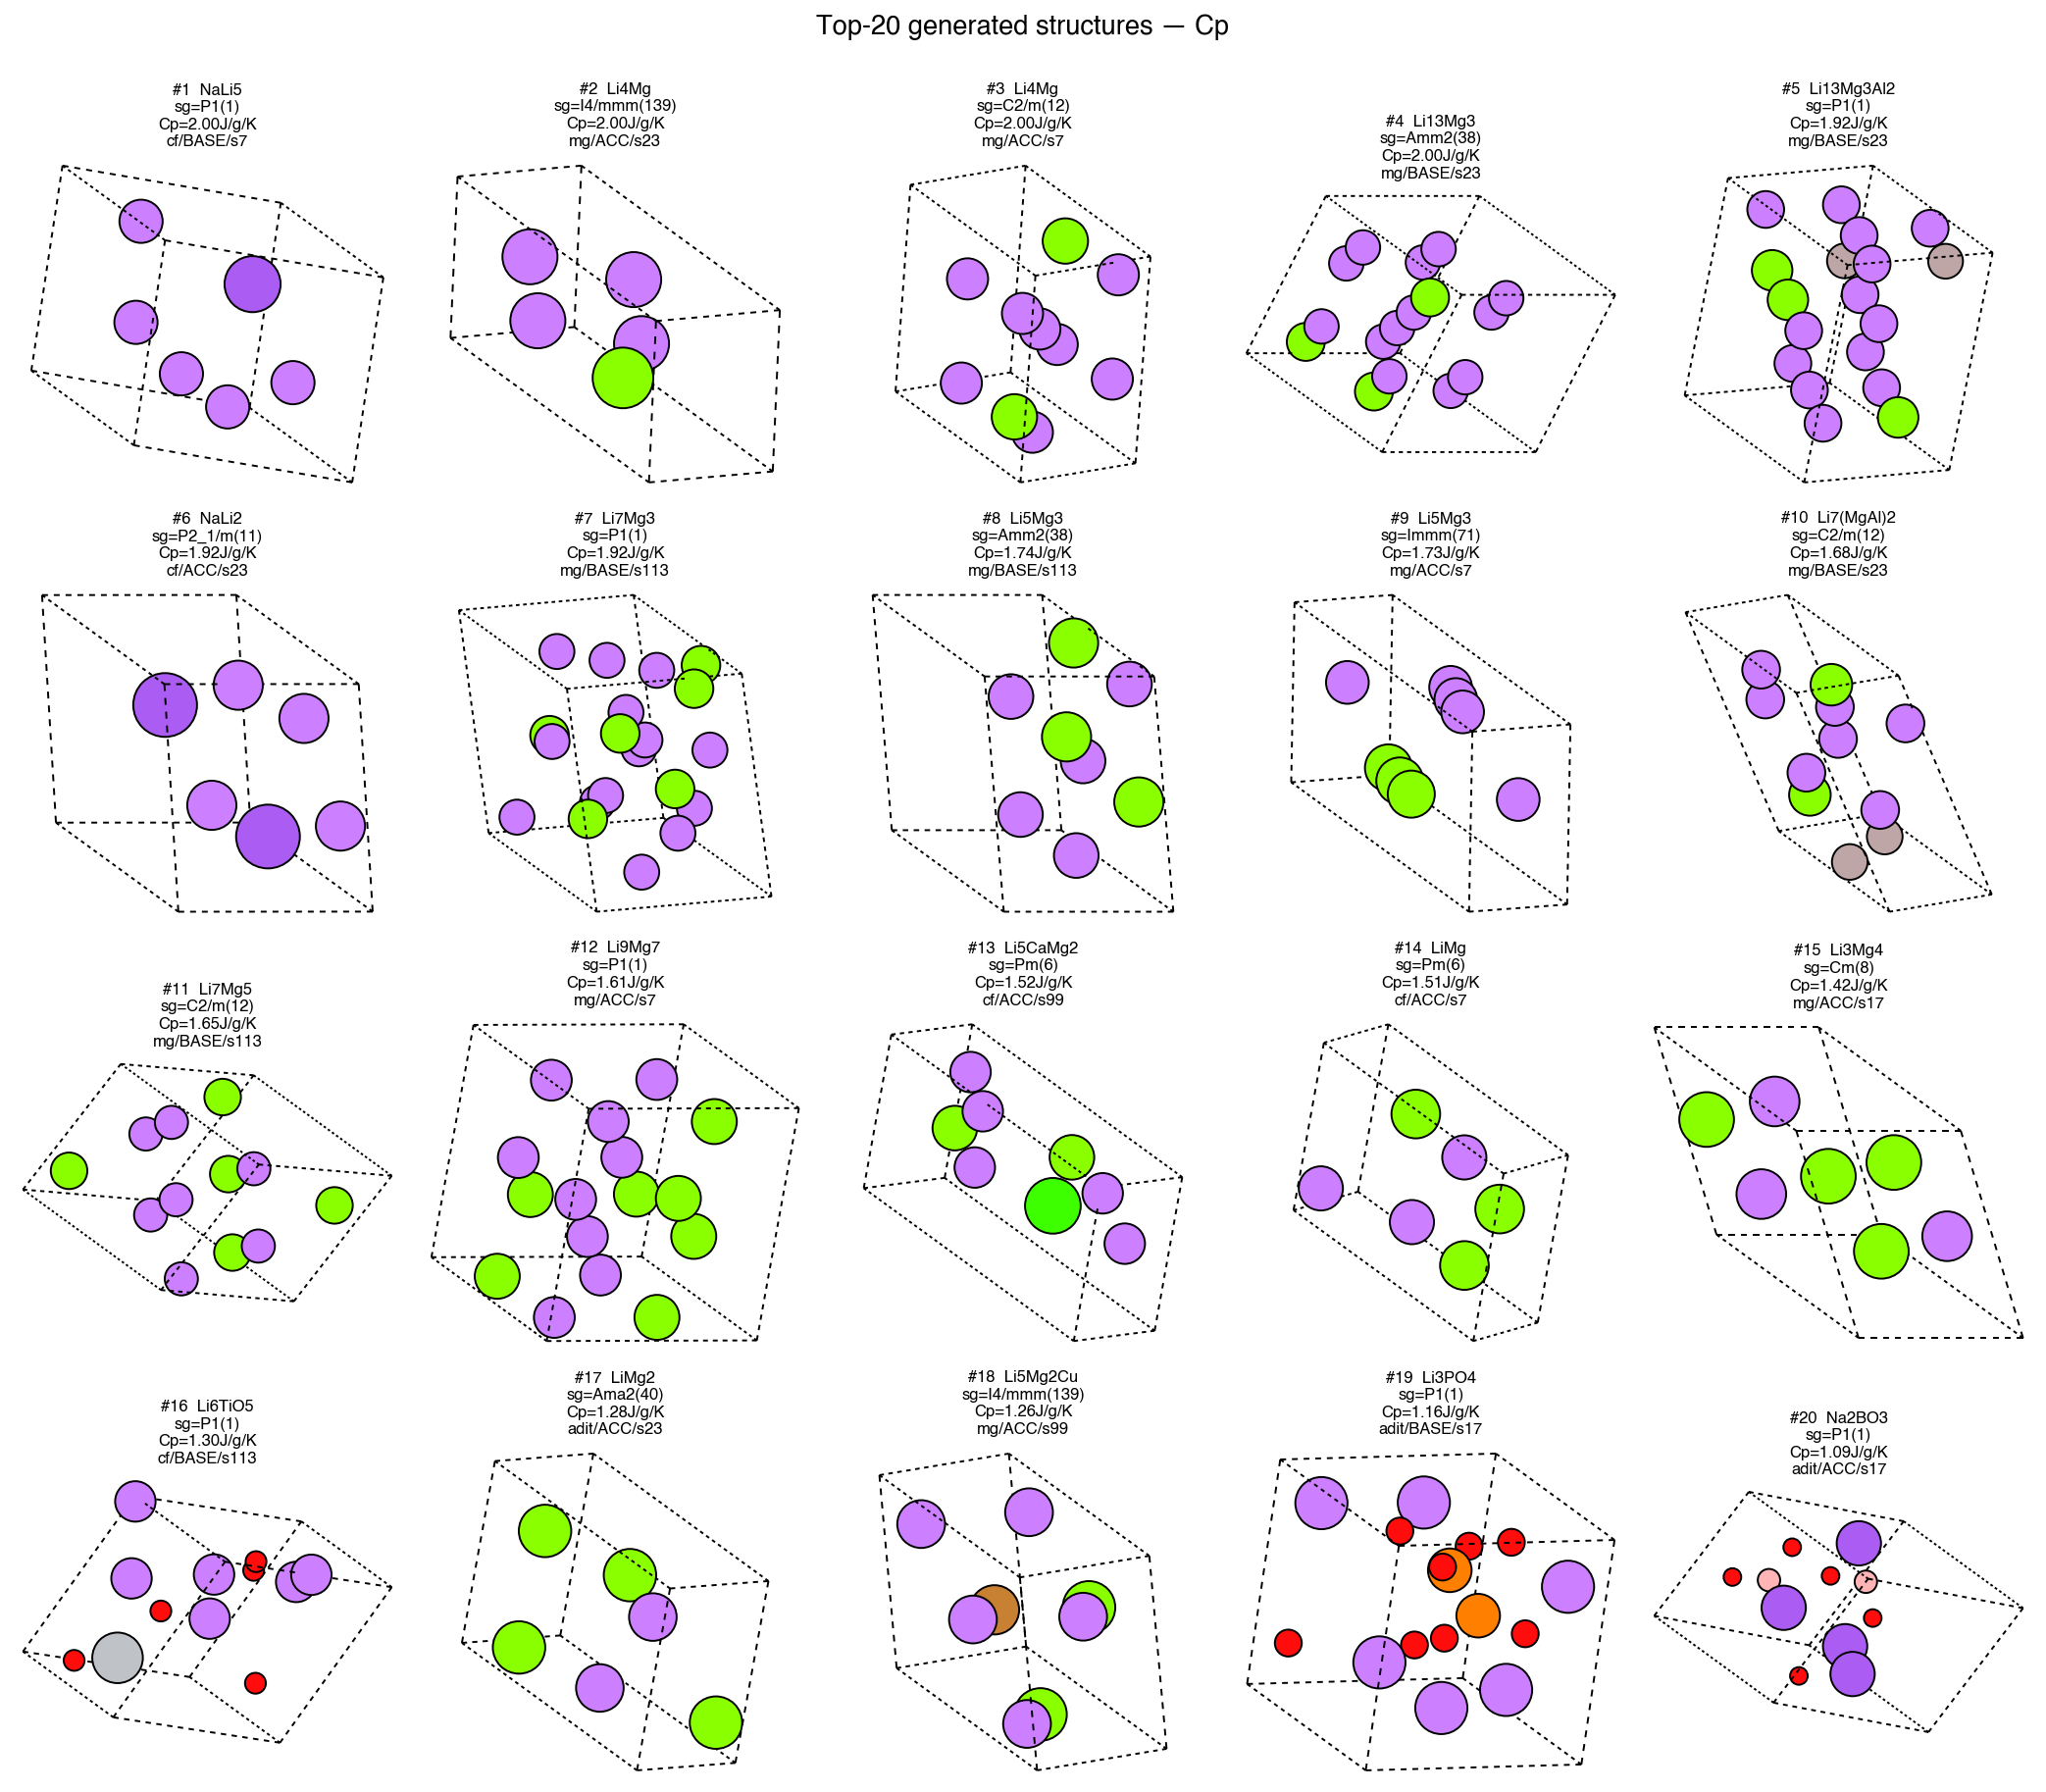
\includegraphics[width=\textwidth]{figures/fig_bogen_structure_zoo_cp.png}
        \caption{Heat capacity ($C_p$)}
    \end{subfigure}
    \hfill
    \begin{subfigure}[t]{0.48\textwidth}
        \centering
        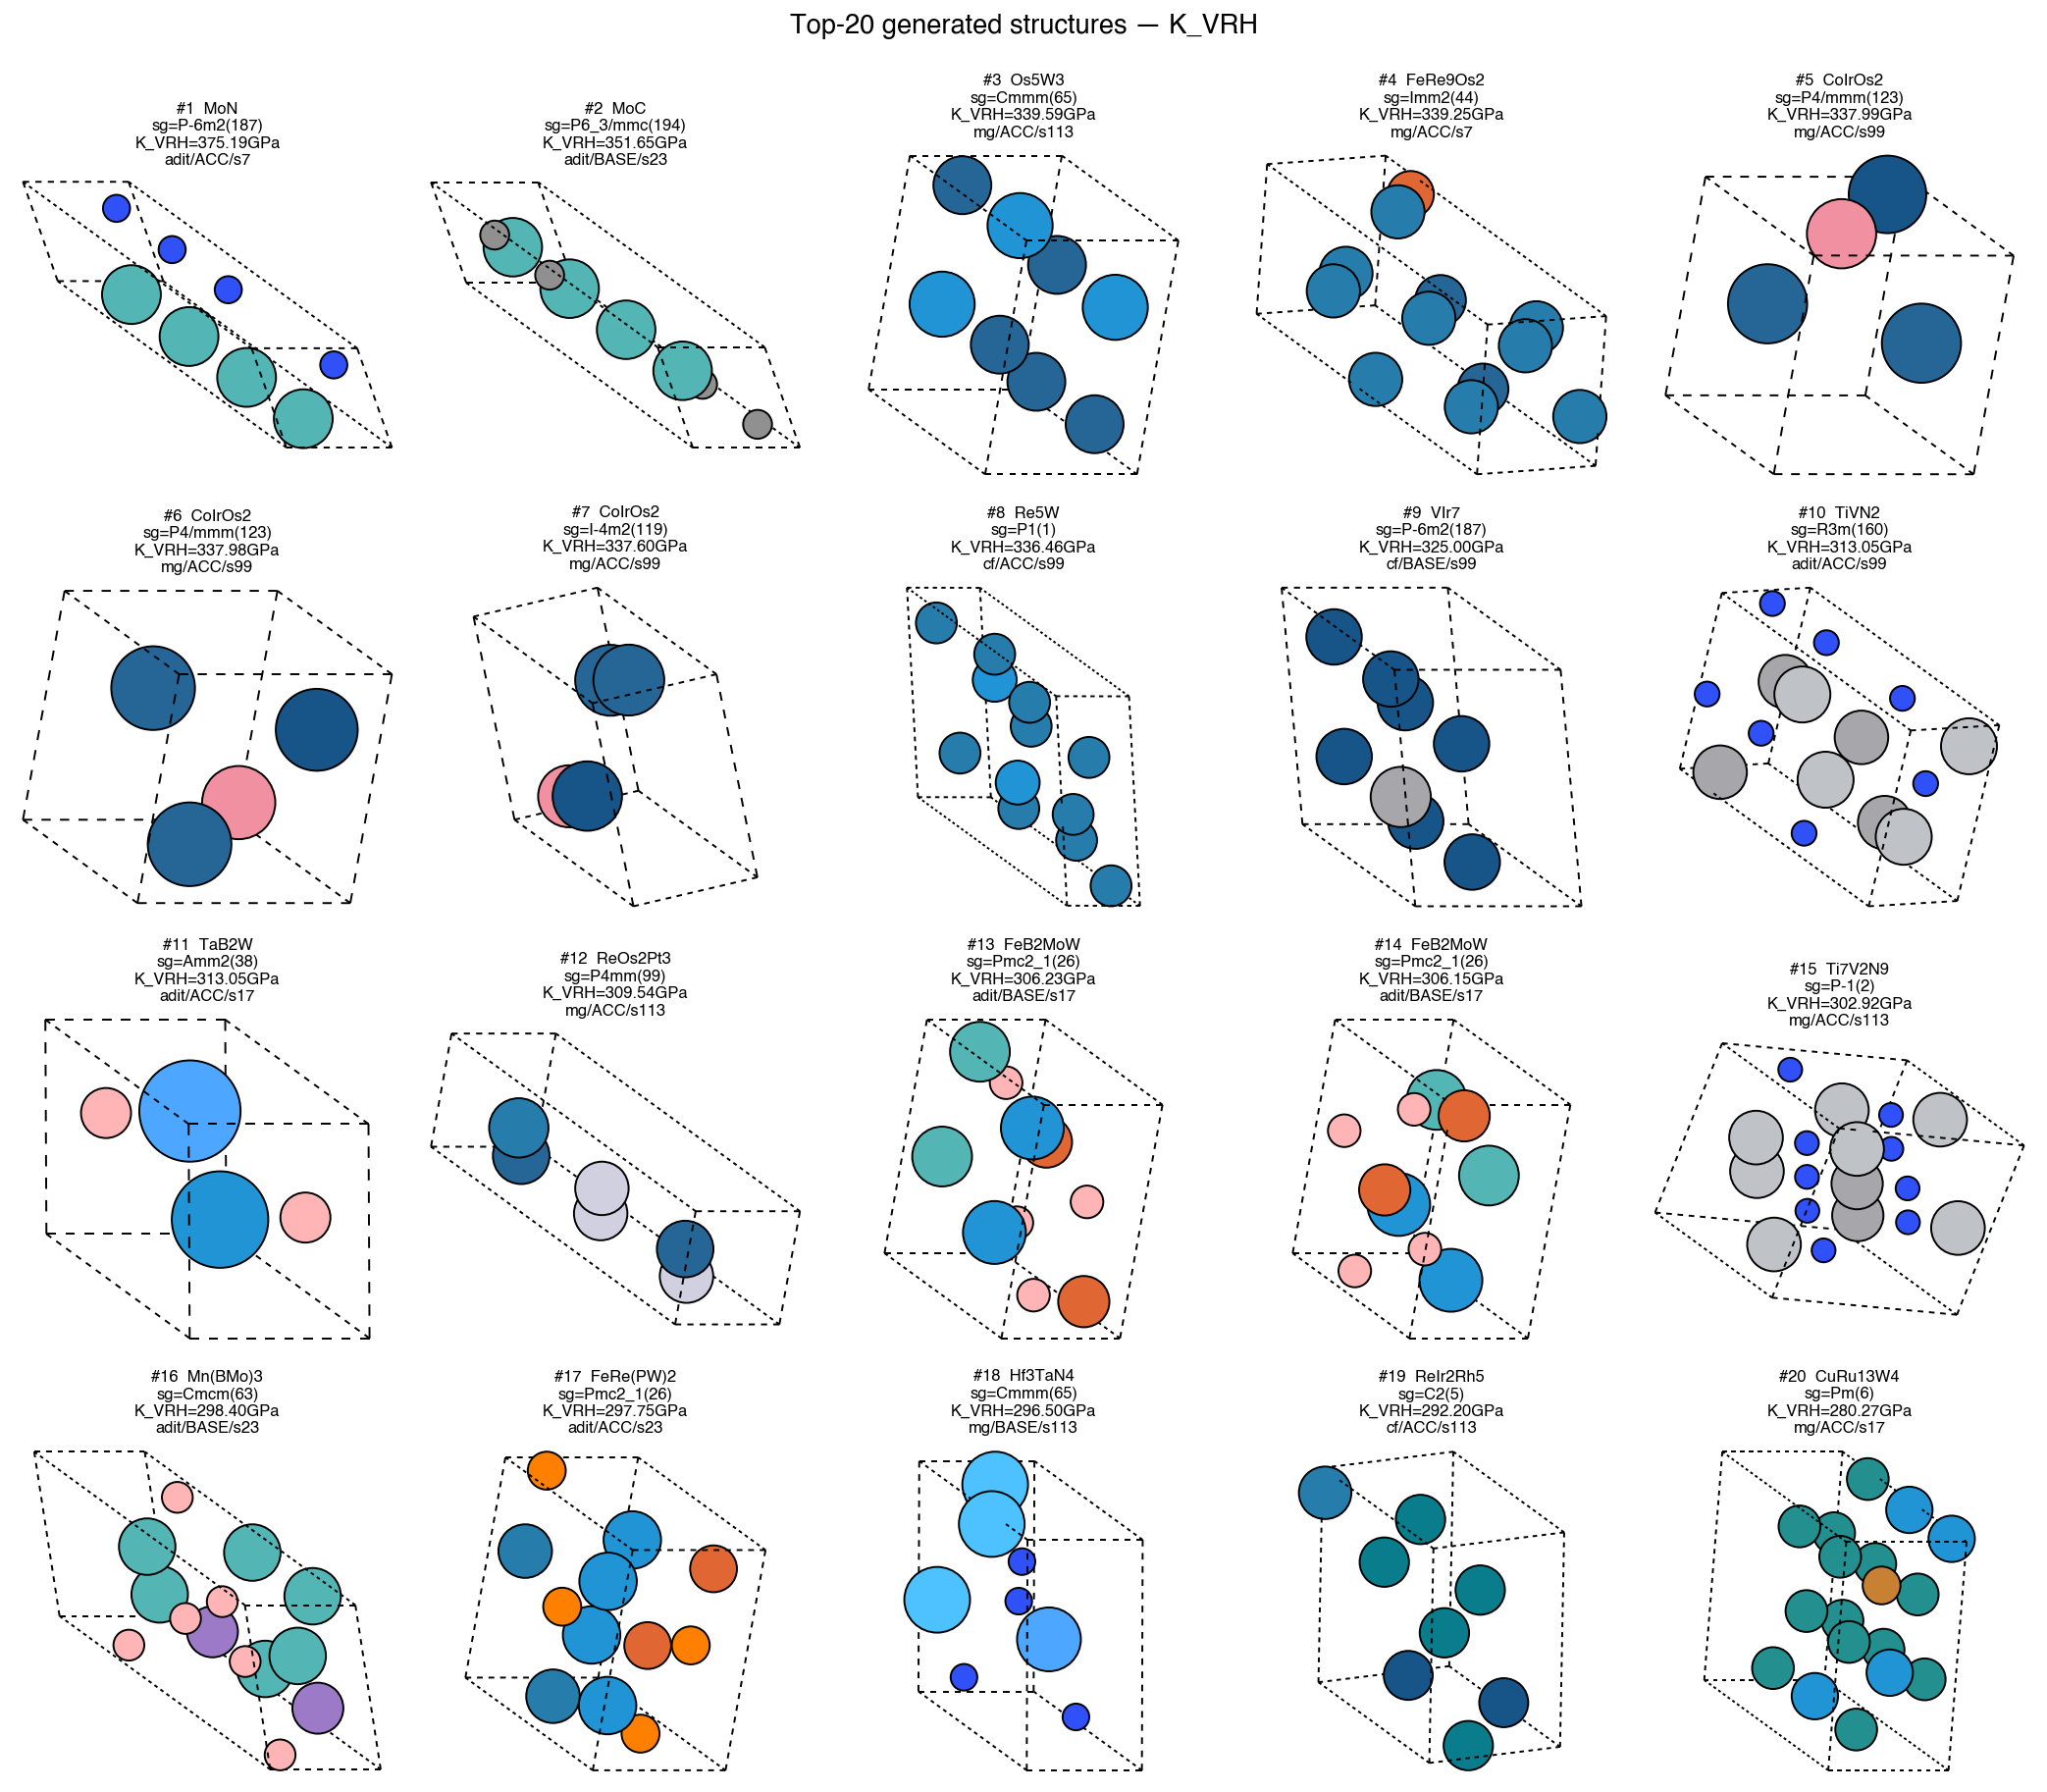
\includegraphics[width=\textwidth]{figures/fig_bogen_structure_zoo_bm.png}
        \caption{Bulk modulus ($K_{\text{VRH}}$)}
    \end{subfigure}
    \caption{Top-20 generated structures per target (4$\times$5 grid), ranked by the oracle. Border colour: blue = MatterGen, green = CrystalFlow, red = ADiT. Each panel reports formula, space group, target value, and the originating (cycle, seed). None pass strict \texttt{StructureMatcher} against the warm-start seed pool.}
    \label{fig:closed_loop_zoo}
\end{figure*}

\subsubsection{What the Probe Does and Does Not Establish}
\label{sec:cl_caveats}

Five seeds, three pretrained backbones, and a learned (not DFT) oracle are enough to draw a few methodological conclusions, not to crown a winning generator.
The loop closes across three architecturally distinct priors with internally self-consistent GP fits across cycles; ACC outperforms BASE in two of three backbones for both targets; the generator does not retrieve memorised seeds; and the crystal-system mix follows each prior's bias.
What the probe does \emph{not} establish is a final ranking of MatterGen vs.\ CrystalFlow vs.\ ADiT.
The cross-seed variance, especially in CrystalFlow, is too large for that, and our oracle is itself a learned surrogate.
A second gap is in the surrogate diagnostics themselves: the only GP-quality signal we log is CV5 on the accumulated training set (Section~\ref{sec:cl_surrogate}), which is a self-consistency check rather than a generalisation test on fresh diffusion proposals.
A definitive comparison would therefore require more seeds per cell, fine-tuning of the diffusion priors against the target property, DFT validation of the top-K hits per backbone, and a held-out RMSE---measured on each cycle's fresh candidates before they reach the gate---to track whether the GP generalises rather than just stays self-consistent.
